\newif\ifsiamonline
\IfFileExists{siamonline250211.cls}{\siamonlinetrue}{\siamonlinefalse}
\ifsiamonline
  \documentclass[review,onefignum,onetabnum]{siamonline250211}
  \newsiamremark{remark}{Remark}
\else
  \documentclass[10pt]{article}
  \usepackage[textwidth=6in,textheight=8in]{geometry}
  \usepackage{amsmath,amssymb,amsthm}
  \usepackage{lmodern}
  \usepackage[mathlines]{lineno}
  \usepackage[colorlinks=true,allcolors=blue!50!black]{hyperref}
  \usepackage{cleveref}
  \linenumbers
  \newtheorem{theorem}{Theorem}[section]
  \newtheorem{lemma}[theorem]{Lemma}
  \newtheorem{proposition}[theorem]{Proposition}
  \newtheorem{corollary}[theorem]{Corollary}
  \theoremstyle{definition}\newtheorem{definition}[theorem]{Definition}
  \theoremstyle{remark}\newtheorem{remark}[theorem]{Remark}
  \newenvironment{keywords}{\par\smallskip\noindent\textbf{Key words.}}{\par}
  \newenvironment{MSCcodes}{\par\smallskip\noindent\textbf{MSC codes.}}{\par}
  \newcommand{\headers}[2]{}
\fi
\usepackage[T1]{fontenc}
\usepackage{xurl}
\usepackage{graphicx,booktabs,array,xcolor}
\usepackage{etoolbox}
% SIAM and fallback statement environments can share a counter.  Supply the
% actual local statement type before that counter is stepped; an alias inside
% an environment is local to its group and does not change the numbering.
\makeatletter
\@ifpackageloaded{cleveref}{}{\usepackage{cleveref}}
\makeatother
\newcommand{\XYstatementtype}[1]{%
  \crefalias{theorem}{#1}%
  \crefalias{lemma}{#1}%
  \crefalias{proposition}{#1}%
  \crefalias{corollary}{#1}%
  \crefalias{definition}{#1}%
  \crefalias{remark}{#1}%
}
\AtBeginEnvironment{theorem}{\XYstatementtype{theorem}}
\AtBeginEnvironment{lemma}{\XYstatementtype{lemma}}
\AtBeginEnvironment{proposition}{\XYstatementtype{proposition}}
\AtBeginEnvironment{corollary}{\XYstatementtype{corollary}}
\AtBeginEnvironment{definition}{\XYstatementtype{definition}}
\AtBeginEnvironment{remark}{\XYstatementtype{remark}}
\crefname{theorem}{theorem}{theorems}
\Crefname{theorem}{Theorem}{Theorems}
\crefname{lemma}{lemma}{lemmas}
\Crefname{lemma}{Lemma}{Lemmas}
\crefname{proposition}{proposition}{propositions}
\Crefname{proposition}{Proposition}{Propositions}
\crefname{corollary}{corollary}{corollaries}
\Crefname{corollary}{Corollary}{Corollaries}
\crefname{definition}{definition}{definitions}
\Crefname{definition}{Definition}{Definitions}
\crefname{remark}{remark}{remarks}
\Crefname{remark}{Remark}{Remarks}
\newcommand{\X}{\mathcal X}
\newcommand{\K}{\mathcal K}
\newcommand{\E}{E_0}
\newcommand{\R}{\mathbb R}
\newcommand{\Z}{\mathbb Z}
\newcommand{\nrm}[1]{\left\lVert#1\right\rVert}
\newcommand{\inner}[2]{\left\langle#1,#2\right\rangle}
\newcommand{\dd}{\mathrm d}
\newcommand{\supp}{\operatorname{supp}}
\newcommand{\dist}{\operatorname{dist}}
\newcommand{\osc}{\operatorname{osc}}
\newcommand{\ind}{\operatorname{ind}}
\newcommand{\diag}{\operatorname{diag}}
\newcommand{\spanof}{\operatorname{span}}
\newcommand{\Pass}{\texttt{PASS}}
\newcolumntype{L}[1]{>{\raggedright\arraybackslash}p{#1}}
\headers{Global annihilation barriers in an infinite lattice}{R. L. Sumoza Matos}
\title{Certified global annihilation barriers in an infinite XY lattice}
\author{Rodolfo Leonardo Sumoza Matos%
  \thanks{Facultad de Ingenier\'ia, Universidad Austral, Pilar, Argentina.
    Departamento de Computaci\'on, Universidad de Buenos Aires, CABA, Argentina.
    Email: \href{mailto:rsumoza@dc.uba.ar}{\nolinkurl{rsumoza@dc.uba.ar}}.
    ORCID: \url{https://orcid.org/0009-0003-3554-4876}.}}
\date{22 October 2026}
\hypersetup{pdftitle={Certified global annihilation barriers in an infinite XY lattice},pdfauthor={Rodolfo Leonardo Sumoza Matos},pdfsubject={Global barrier certification, effective local input class, and coupling robustness}}
\begin{document}
\maketitle
\begin{abstract}
A numerical saddle does not establish a globally optimal escape route. We certify the annihilation barrier of a neutral dipole at separation twelve in the exact-cosine XY model on the infinite square lattice. Admissible paths are strongly continuous in the homogeneous energy space and end at any physical uniform phase lift. A finite atlas with rigorous control of infinite-dimensional transverse fibers separates a local minimum from every endpoint. Exact-saddle caps and a validated upper path identify the barrier with an asymmetric index-one saddle height relative to the minimum. In unit-coupling normalization, the barrier lies strictly between 0.00567867 and 0.00570116. Reusable a posteriori tests cover signed-bond coercivity, full dual residuals, and complete boundary coverage. An explicit lattice Green estimate controls critical-state and path tails. Subcritical connections then reuse the global certificate on an infinite class of noncompact initial perturbations with prescribed block tails. We prove termination of barrier enclosures at any requested precision on this class, without claiming a general search implementation. Under summable coupling perturbations of total norm at most 0.002, the minimum and two index-one saddles persist and the global barrier remains positive; the continued saddles are not identified as perturbed minimax realizers. Frozen sources and a fresh execution record document the fixed global certificate. Completeness for arbitrary XY configurations remains open.
\end{abstract}
\begin{keywords}
XY lattice, annihilation barrier, computer-assisted proof, index-one saddle, a posteriori verification, lattice Green function
\end{keywords}
\begin{MSCcodes}
82B20, 49J35, 65G20
\end{MSCcodes}

\section{Introduction}\label{sec:intro}

Discrete phase models support pinned defects, saddle-mediated transitions, and competing escape paths. Finding one path with a low energy maximum gives an upper bound on an activation barrier. Proving that this path is globally optimal requires excluding every less expensive path, including those that leave a proposed reaction surface or create additional defects. On an infinite lattice, even a very accurate finite-box saddle leaves an exterior verification problem. A small residual at the interior vertices does not control the residual created at the interface of an extension.

This paper addresses that distinction for a neutral dipole in the square-lattice XY model with the exact interaction $1-\cos t$. We work in the homogeneous energy Hilbert space $\X$ defined in \cref{sec:model}. Our central result identifies the annihilation barrier over \emph{all} strongly $\X$-continuous paths to any physical uniform lift. It is a variational assertion about the full infinite lattice, rather than a minimum within a frozen two-coordinate family.

\subsection{Results and their scope}

For a dipole with charges $+1$ and $-1$ at plaquettes $(0,0)$ and $(12,0)$, the computation certifies a minimum $m_0$ and two reflected asymmetric index-one saddles $s_+$ and $s_-$. Their common energy is denoted by $h$. An open bounded set $\mathcal D\subset\X$ contains $m_0$, excludes every annihilation endpoint from its closure, and satisfies $\E\ge h$ on its entire boundary. A separately validated path from $m_0$ to an endpoint has maximum $h$. Consequently,
\begin{equation}\label{eq:intro-barrier}
 B_0(m_0)=h-\E(m_0),\qquad
 0.00567867<B_0(m_0)<0.00570116.
\end{equation}
Here the coupling is one, and the numbers are dimensionless. The minimum and saddle assertions refer to general perturbations in $\X$; no symmetry restriction or positivity of every core bond is imposed. The meaning of ``all paths'' includes the specified strong topology and the endpoint set in \cref{eq:barrier}.

The geometric argument becomes reusable through \cref{thm:certificate}. Its hypotheses are a finite collection of rigorous inequalities, together with analytic formulas controlling the exterior. The conditions cover full dual residuals, signed-bond coercivity, saddle index, exact cutting planes, transverse fibers, all chart faces and seams, and endpoint attachment of the upper path. A certificate that fails one test is inconclusive; it does not prove instability or absence of a lower route. The verification format permits adaptation to another instance without asserting that the search for a successful certificate always terminates.

Three analytic extensions complement this fixed example. First, \cref{thm:green} gives an explicit Fourier estimate for the orthogonal projection onto lattice gradients. Combined with the stationary equation, it yields an inverse-radius energy tail. Its constants also control the already validated upper path. Second, \cref{thm:local-class,thm:class-termination} reuse the fixed
communication height for an explicit infinite class of initial fields.
The class is generated by compact rational blocks with a geometric
norm budget and a prescribed spatial support sequence. It allows
noncompact perturbations without imposing symmetry. A subcritical
connection to $m_0$ transfers the full path-space certificate, and a
constructive energy enclosure terminates for every rational accuracy.
This is a consequence of the existing global certificate, rather than a
search for all mechanisms. The general refinement procedure is proved;
the new code checks its constants and representative finite prefixes.
Third, \cref{thm:robustness} treats the infinite-dimensional family of interactions
\begin{equation}\label{eq:intro-perturbation}
 E_b(\theta)=\sum_e(1+b_e)(1-\cos D_e\theta),\qquad
 b\in\ell^1(\mathcal E),\quad\nrm b_1\le 1/500.
\end{equation}
The minimum and the two distinct index-one saddles continue, the minimum retains its charges, and
\begin{equation}\label{eq:intro-robust}
 |B_b(m_b)-B_0(m_0)|\le2\nrm b_1.
\end{equation}
Thus the perturbed global barrier remains strictly positive. The same coupling class admits a uniform inverse-radius tail for the three continued critical states. We also prove local exponential stability for the specified energy-space gradient flow. We do not claim that a continued saddle necessarily realizes the perturbed minimax, or that a mechanism switch has been established.

\subsection{Relation to prior work}

Certification of critical points of cosine energy landscapes is established. Mehta, Hauenstein, and Wales \cite{Mehta2014} used algebraic certification for finite XY systems with periodic or antiperiodic boundaries. More recently, Ayala, Choksi, and Wirth \cite{Ayala2026} validated finite atomistic configurations and transition-state candidates. These results show why neither an XY critical point certificate nor a validated finite-dimensional saddle should be presented as the new conclusion here.

Metastability and depinning for square-lattice systems with periodic interactions, including XY models, were studied variationally by Alicandro, De Luca, Garroni, and Ponsiglione \cite{Alicandro2014}. They established metastable configurations and derived vortex dynamics through minimizing movements and continuum-limit arguments. Here the lattice spacing and the vortex separation are fixed, and the quantity to be certified is the global communication height from a specified metastable state over all strong energy-space escape paths.

For lattice defects, Hudson and Ortner \cite{Hudson2015} obtained strongly stable multi-dislocation configurations from an isolated-core stability hypothesis and sufficient separation. We verify a particular dipole equilibrium and a global escape barrier at a fixed separation. Hudson \cite{Hudson2017} derived asymptotic energy barriers in a finite-domain, piecewise-quadratic dislocation model with a specified single-hop path class. Garroni, Petrache, and Spadaro \cite{Garroni2025} proved clearing-out results for global minimizers of discrete energies with topological singularities. Global minimization and pinned local metastability ask different questions; a clearing-out theorem does not supply a continuous path with a prescribed ceiling from a given metastable state.

Validated transition paths also have direct precedents. Breden and Kuehn \cite{Breden2019} rigorously validated saddle connections in a stochastic transition-path setting. Liu, Chen, and Ortner \cite{Liu2024} developed stability theory for minimum energy paths in Hilbert spaces under explicit nondegeneracy hypotheses. Berglund, Medvedev, and Simpson \cite{Berglund2025} analyzed metastability and relevant transition barriers in the finite one-dimensional nearest-neighbor Kuramoto model, also a cosine system. These works preclude a general claim of priority for a saddle-height formula, for infinite-dimensional path theory, or for rigorous transition geometry. Our lower bound instead comes from a complete separating boundary in the energy space of a two-dimensional infinite lattice. It does not assume that a previously selected path is a minimum energy path.

Several ingredients of the certificate also have established analogues. A posteriori existence arguments based on computable residuals and stability bounds have a substantial history; see Ortner \cite{Ortner2009} for an inverse-function framework for nonmonotone problems. Signed Laplacian positivity and inertia can be expressed through Schur complements and effective resistances \cite{Chen2020}. Cubical sublevel computations and their verification are treated by D\l{}otko and Wanner \cite{Dlotko2018}.

Far-field estimates and boundary approximations were developed by Ehrlacher, Ortner, and Shapeev \cite{Ehrlacher2016}. Braun, Hudson, and Ortner \cite{Braun2022} obtained systematic far-field expansions using continuum correctors and discrete multipoles; higher-order boundary conditions were subsequently developed by Braun, Ortner, Wang, and Zhang \cite{Braun2025} and by Wei, Braun, Wang, and Zhang \cite{Wei2026}. For the present certificate we require explicit constants in matching bond conventions for the critical states and for an entire upper path.

The contribution is therefore a specific conjunction: the exact cosine interaction on the infinite square lattice; unrestricted strong energy-space escape paths; a matched global lower and upper barrier bound; checkable hypotheses exposing the infinite-dimensional reduction; a terminating reuse procedure on a specified infinite input class; and a quantitative perturbation theorem with effective tails in the same coupling class. We do not infer from this comparison that earlier methods are incapable of adaptation, nor assert universal bibliographic priority.

\subsection{Verification record and organization}

The numerical theorem uses frozen proposals and rigorous verification, with the three source archives indexed in the supplementary record. A fresh execution of the standard supervisor reproduced every phase it invokes, without using cached validated outputs as mathematical premises. This is a reproduction of the same verification software, supported by analytic review; it is not an independent interval implementation or a proof-assistant formalization. The reproducibility record distinguishes these levels of evidence.

\Cref{sec:model} fixes the topology and normalization. \Cref{sec:certificate} gives the reusable a posteriori theorem, and \cref{sec:instance} records its verified instance. \Cref{sec:green,sec:local-class,sec:robustness} prove the effective-tail, terminating local-class, and coupling-robustness extensions. \Cref{sec:discussion} discusses algorithmic scope and the next certification problem.

\section{Energy space, lifts, and normalization}\label{sec:model}

Let $V=(\Z+\tfrac12)^2$ and orient each nearest-neighbor bond in a positive coordinate direction; $\mathcal E$ contains each undirected bond exactly once. Write $D_eu=u(y)-u(x)$ for $e=(x,y)$. Define the closed gradient subspace first:
\[
 \mathcal G=\overline{\{D\varphi:\varphi\in C_c(V;\R)\}}^{\,\ell^2(\mathcal E)}.
\]
The homogeneous energy space and its energy are
\begin{equation}\label{eq:energy-space}
 \inner uv_\X=\sum_e D_euD_ev,\qquad
 \X=\{u:V\to\R:Du\in\mathcal G\}/\R,
 \qquad\E(u)=\sum_e(1-\cos D_eu).
\end{equation}
The quotient identifies vertex representatives differing by a constant.
The map $D:\X\to\mathcal G$ is an isometric isomorphism: each
$g\in\mathcal G$ has zero oriented sum around every finite cycle, since
finite-cycle sums are continuous on $\ell^2(\mathcal E)$ and vanish on
compact gradients. Integrating $g$ along finite lattice paths therefore
reconstructs a vertex representative, unique modulo a constant.
Thus $\X$ is a Hilbert space, equivalently the homogeneous completion of
compactly supported vertex fields represented modulo constants. Finite-path
vertex differences are continuous in its norm. The energy is finite,
nonnegative, and at most $\nrm u_\X^2/2$.

The physically uniform configurations and admissible barriers are
\begin{align}
 \K&=\{u\in\X:D_eu\in2\pi\Z\text{ for every }e\},\label{eq:vacua}\\
 B_b(u)&=\inf_{\substack{\gamma\in C([0,1];\X)\\
                 \gamma(0)=u,\ \gamma(1)\in\K}}
     \max_{t\in[0,1]}\{E_b(\gamma(t))-E_b(u)\}.\label{eq:barrier}
\end{align}
Write $B_0$ when $b=0$. Replacing the endpoint set by the single representative zero can change the stated problem. Each energy is invariant under addition of an element of $\K$.

Every nonzero $k\in\K$ satisfies $\nrm k_\X\ge4\pi$. Indeed, its integer gradient has finite support, and a nonconstant integer field has at least four bonds with nonzero difference on the square lattice. Thus the quotient map $\X\to\X/\K$ is a local isometry and continuous paths lift uniquely after an initial lift is fixed, by subdividing the compact time interval into neighborhoods smaller than half this separation. Consequently \cref{eq:barrier} also describes paths to the physical vacuum in the phase quotient. Convergence on every fixed finite box is a weaker topology: translating a defect to infinity does not supply a strong energy-space path ending at the vacuum.

We use the Riesz gradient $F(u)=\nabla_\X\E(u)$ and its self-adjoint derivative $H(u)$. The basic differential facts will also specify the constants used in the verification.

\begin{lemma}\label{lem:basic}
The energy is smooth on $\X$, and
\begin{align}
 \inner{F(u)}v_\X&=\sum_e\sin(D_eu)D_ev,\label{eq:firstvar}\\
 \inner{H(u)v}w_\X&=\sum_e\cos(D_eu)D_evD_ew.\label{eq:hessian}
\end{align}
The bond evaluation functional has norm $1/\sqrt2$. In particular,
\begin{equation}\label{eq:basic-bounds}
 \nrm{H(u)}\le1,\qquad
 \nrm{H(u)-H(v)}\le\Lambda\nrm{u-v}_\X,
 \qquad \Lambda=1/\sqrt2.
\end{equation}
For $h\in\X$, the gradient and energy Taylor remainders are bounded by
\begin{gather}\label{eq:remainders}
 \nrm{F(u+h)-F(u)-H(u)h}\le\tfrac\Lambda2\nrm h_\X^2,\qquad\qquad
 \nonumber\\
 |\E(u+h)-\E(u)-\inner{F(u)}h_\X
          -\tfrac12\inner{H(u)h}h_\X|
       \le\tfrac\Lambda6\nrm h_\X^3.
\end{gather}
\end{lemma}
\begin{proof}
The Fourier isometry sends a lattice gradient to $d(k)\widehat u(k)$, with $d_j=e^{ik_j}-1$ and $|d|^2=4-2\cos k_1-2\cos k_2$. The squared norm of one bond evaluation is the normalized torus integral of $|d_j|^2/|d|^2$. The two integrals agree by coordinate exchange, and their sum is one, so each is $1/2$. The value at $k=0$ does not affect the integral. This also follows from the projection construction in \cref{sec:green}.

Since $|\sin t|\le|t|$, the first variation defines a bounded functional. Cauchy--Schwarz gives $\nrm{H(u)}\le1$, and
\[
 |\inner{(H(u)-H(v))a}c_\X|
 \le\nrm{D(u-v)}_\infty\nrm a_\X\nrm c_\X
 \le\Lambda\nrm{u-v}_\X\nrm a_\X\nrm c_\X.
\]
The same estimate bounds the trilinear third derivative by $\Lambda$. For every $j\ge2$, placing two gradient factors in $\ell^2$ and the other $j-2$ factors in $\ell^\infty$ bounds the $j$th derivative by $\Lambda^{j-2}\prod_{i=1}^j\nrm{v_i}_\X$; the same coefficient-continuity argument proves smoothness. Differentiation follows by dominated remainder estimates on the bond sums; continuity follows from uniform convergence of the coefficient increments in $\ell^\infty$. Integration along a line gives \cref{eq:remainders}.
\end{proof}

At the vacuum, $H(0)=I_\X$. A coercivity estimate here is measured against $\nrm{Dv}_2^2$, not against the vertex $\ell^2$ norm. The local vertex Laplacian has spectrum touching zero on the infinite lattice, so this energy-space gap is not an $\ell^2$ spectral gap.

For a plaquette $p$, choose principal bond increments in $(-\pi,\pi)$ and take their oriented sum divided by $2\pi$. If no increment is at a branch endpoint, this defines an integer charge $q_p$. A uniform margin from those endpoints and the bond evaluation bound certify charge preservation under energy-norm corrections. The dipolar state in \cref{sec:instance} has finite total energy and exactly two nonzero charges. We use this charge statement only after its global branch and exterior checks, not as an assumed constraint on escape paths.

\subsection{Dissipation metric and dynamical interpretation}

The choice of metric specifies how the phase field dissipates energy. In
this paper the dissipation potential for an instantaneous velocity $v$ is
\[
 \mathcal R(v)=\frac12\sum_e|D_ev|^2
             =\frac12\nrm v_\X^2.
\]
Thus the velocity is the unique minimizer of
$\mathcal R(v)+DE_b(u)[v]$ over $\X$. Its Euler equation is
\begin{equation}\label{eq:flow}
 \dot u=-\nabla_\X E_b(u).
\end{equation}
Its weak form is
\begin{equation}\label{eq:flow-weak}
 \sum_eD_e\dot u\,D_ev
       =-\sum_e(1+b_e)\sin(D_eu)D_ev
       \quad(v\in\X).
\end{equation}
Writing $D^*$ for the adjoint from bond fields to vertex distributions,
this is $D^*D\dot u=-D^*((1+b)\sin Du)$, understood weakly. Along a
solution,
\[
 \frac{\mathrm d}{\mathrm dt}E_b(u(t))
   =-\nrm{\dot u(t)}_\X^2=-\sum_e|D_e\dot u(t)|^2.
\]
The metric therefore measures dissipation through differences of phase
velocities across bonds, rather than through independent vertex velocities.

This interpretation has a circuit realization. In a finite array of
overdamped resistively shunted Josephson junctions with equal shunt
conductances, a bond voltage is proportional to its phase difference
velocity. After nondimensionalizing, the sum of the resistive and
Josephson bond currents has the form
$i_e=D_e\dot u+J_e\sin(D_eu)$, where $J_e=1+b_e$.
Kirchhoff conservation at every free vertex gives $D^*i=0$ in the absence
of injected current and noise, which is the weak equation above when
the boundary phases are held fixed. The homogeneous current-conservation
equation is given in \cite[Eq.~(13)]{Yoon2000}; fluctuating twists require
the additional equations specified there and are not included here.
The corresponding Joule dissipation is proportional to
$\sum_e|D_e\dot u|^2$. On the infinite lattice we use the finite-energy
weak formulation itself, rather than assuming a thermodynamic limit of
the driven or noisy finite-array model. In particular, no bounded
inverse of the vertex Laplacian on $\ell^2$ is asserted.

The barrier theorem and the dynamical corollary answer distinct questions.
The barrier is determined by the energy and the admissible strong-$\X$
path class in \eqref{eq:barrier}; changing the mobility while keeping
those two objects fixed does not change this variational quantity.
The flow above provides a specified dissipative relaxation model and
the local stability assertion in \cref{cor:flow}. An energy barrier alone
does not validate a connecting orbit, a thermal escape rate, or the
thermodynamic Berezinskii--Kosterlitz--Thouless transition. A different
mobility, noise law, or path topology requires its own dynamical analysis.

\section{A posteriori global-barrier certificates}\label{sec:certificate}

We give sufficient conditions whose numerical content consists of finite
matrix inequalities, scalar interval bounds, and a finite boundary ledger.
The conditions apply to the full space $\X$. Their verification does not
restrict perturbations to a symmetry class or identify a finite-box
Hessian with its infinite-lattice counterpart. Throughout this section,
$F=\nabla_\X\E$, $H_\theta=DF(\theta)$, and
$\Lambda=1/\sqrt2$ is the Hessian Lipschitz constant from
\cref{lem:basic}. The weaker bound $\Lambda=1$ may instead be used
in an individual numerical estimate when its sufficient inequalities still
hold. In particular, the correction estimates below allow that coarser
choice; the displayed cap parameters use the sharp bound, or its rational
upper bound $71/100$.
Unmarked norms and pairings are those of $\X$, with induced operator
norms; finite coordinate vectors carry their Euclidean norm.

The input representation matters. Each candidate is a specified analytic
finite-energy reference plus a compact dyadic correction. Its exterior
energy, force, branch, and edge-increment remainders must have proved
bounds. All core--exterior interface bonds are included. Finite arrays
alone do not certify a full $\X^*$ residual. The construction below is an
a posteriori criterion for such represented data, rather than an
algorithm guaranteed to succeed for every configuration.

\subsection{Full-space coercivity from finite matrices}

Let $Q:\R^d\to\X$ have linearly independent compact columns
$q_1,\ldots,q_d$, and write
\begin{equation}\label{eq:cert-projections}
 G=Q^*Q,\qquad P_Q=QG^{-1}Q^*,\qquad Y=\ker Q^*.
\end{equation}
The case $d=0$ means $Y=\X$ and no deflation. The projection is exact;
an approximate normalization of stored columns is not substituted for $G$.

\begin{lemma}[Neumann comparison]\label{lem:cert-neumann}
Let $f$ be an algebraically zero-mean vertex load supported in a square
of $N\times N$ vertices, $N\ge2$. Let $L_N$ count only bonds interior to that
square. If $f^\sharp$ denotes its Riesz representative in $\X$, then
\begin{equation}\label{eq:cert-neumann}
 \nrm{f^\sharp}^2\le f^TL_N^\dagger f,
 \qquad
 \left|f^TL_N^\dagger f-f^Tu\right|
 \le \|f\|_{\ell^2}\frac{N^2}{4}\|f-L_Nu\|_{\ell^2}
\end{equation}
for every finite proposal $u$. No mean constraint on $u$ is required.
\end{lemma}
\begin{proof}
In the variational formula
$\nrm{f^\sharp}^2=\sup_v(2f[v]-\nrm{v}^2)$, discard all bonds not
interior to the square. The supremum increases to the finite Neumann
problem. The constant mode causes no obstruction because $f$ has zero
mean. Moreover,
$\lambda_1(L_N)=4\sin^2(\pi/(2N))\ge4/N^2$.
Choose a solution $u_*$ of $L_Nu_*=f$ with the same mean as $u$.
Then $\|u_*-u\|_{\ell^2}\le N^2\|f-L_Nu\|_{\ell^2}/4$, which proves the
second inequality by pairing with $f$.
\end{proof}

The square in this lemma must contain the complete load, including both
endpoints of every nonzero flux bond used to form its divergence. The
inequality is an upper comparison; it gives no lower bound on the
infinite dual norm. Mutual load pairings can be enclosed by the same
finite solves and residual bounds. A separately proved residual
remainder $D^*r$, with $\|r\|_{\ell^2}\le\varepsilon$, contributes
at most $\varepsilon$ to the dual norm.

For the fixed neutral dipole used below, Appendix~\ref{app:reflected-residual}
proves the finite load's zero mean by compact-flux cancellation and reflection
of the analytic reference, without assuming symmetry of the saddle correction.
It also derives the explicit exterior dual remainder and includes the
core--exterior interface. Thus the mean condition in
\cref{lem:cert-neumann} is checked algebraically for these inputs.

\begin{proposition}[Deflated signed-resistance test]\label{prop:cert-gram}
Suppose, uniformly over a prescribed set of configurations,
\begin{equation}\label{eq:cert-deficits}
 H_\theta[v,v]\ge a_0\nrm{v}^2
       -\sum_{e\in S}W_e|D_ev|^2,\qquad a_0>0,\quad W_e\ge0,
\end{equation}
where $S$ is finite. A containing Neumann square includes both endpoints
of every bond in $S$ and the complete supports of $Q$, whose columns
vanish on its boundary. Let
$R_N=(f_e^TL_N^\dagger f_f)_{e,f\in S}$, where
$f_e=\delta_{e^+}-\delta_{e^-}$, and let $B_{ej}=D_eq_j$.
If the finite matrix inequality
\begin{equation}\label{eq:cert-matrix-test}
 W^{1/2}(R_N-BG^{-1}B^T)W^{1/2}
       \preceq a_0\kappa I,\qquad \kappa<1,
\end{equation}
is verified, then $H_\theta|_Y\succeq\mu I$ on the full infinite
complement, where $\mu=a_0(1-\kappa)>0$.
\end{proposition}
\begin{proof}
The infinite trace Gramian restricted to $Y$ is
$R_\infty^Y=R_\infty-BG^{-1}B^T$. Applying
\cref{lem:cert-neumann} to every linear combination of the loads gives
$R_\infty\preceq R_N$. Thus the norm squared of the weighted trace
map $v\mapsto (\sqrt{W_e}D_ev)_{e\in S}$ on $Y$ is at most
$a_0\kappa$. Substitution in \eqref{eq:cert-deficits} proves the claim.
The zero boundary values of the reaction columns ensure that their
finite and infinite energy products agree.
\end{proof}

The test uses the entire matrix, including mutual resistances. A
validated congruence using interval enclosures of all its entries is
sufficient. Individual diagonal resistance tests are not equivalent.
Finite signed-Laplacian reductions have substantial precedents
\cite{Chen2020}; the role of \cref{prop:cert-gram} here is to preserve
the direction of the comparison with the infinite complement.

The weights in \eqref{eq:cert-deficits} are obtained from interval
enclosures of $\cos(D_e\theta)$, with an analytic positive floor outside
$S$. For a chart displacement $w\in Y$, $\nrm{w}\le R$, the sharper
edge estimate
\begin{equation}\label{eq:cert-deflated-edge}
 |D_ew|\le R\sqrt{\tfrac12-b_e^TG^{-1}b_e},
 \qquad b_e=(D_eq_1,\ldots,D_eq_d)^T,
\end{equation}
follows by subtracting the projection of the edge evaluation functional.
It is used before enclosing the trigonometric weights. Negative core
bonds are allowed; positivity is required of the resulting form.

\subsection{Critical points and exact saddle planes}

\begin{lemma}[Frozen Newton and Morse index]\label{lem:cert-newton}
Let $\widehat\theta\in\X$ and $\nrm{F(\widehat\theta)}\le\delta$.
Assume either $H_{\widehat\theta}\succeq\gamma I>0$, or there is a unit
$q\in\X$ such that
\begin{equation}\label{eq:cert-saddle-splitting}
 H_{\widehat\theta}[q,q]\le-a<0,\qquad
 H_{\widehat\theta}|_{q^\perp}\succeq c_{\perp}I>0,
 \qquad \gamma=\min(a,c_{\perp}).
\end{equation}
If
\begin{equation}\label{eq:cert-newton-radius}
 \delta+\tfrac\Lambda2\rho^2\le\gamma\rho,
 \qquad \Lambda\rho<\gamma,
\end{equation}
there is a unique critical point $\theta_*$ in
$\overline B_\X(\widehat\theta,\rho)
 =\{u:\nrm{u-\widehat\theta}_\X\le\rho\}$. It is a strict minimum in the
first case and has Morse index one in the second. Its Hessian inverse
has norm at most $(\gamma-\Lambda\rho)^{-1}$.
\end{lemma}
\begin{proof}
In the saddle case write $v=tq+y$ and set $Jv=-tq+y$. Self-adjointness
cancels the cross terms:
\[
 \inner{H_{\widehat\theta}v}{Jv}
 =-t^2H_{\widehat\theta}[q,q]+H_{\widehat\theta}[y,y]
 \ge\gamma\nrm{v}^2.
\]
Lax--Milgram applied to $JH_{\widehat\theta}$ gives an inverse bounded
by $1/\gamma$. The positive $q^\perp$ block has a negative scalar
Schur complement, so its Morse index is exactly one. No smallness
assumption on the off-diagonal block is needed. In the minimum case
the inverse bound is immediate. The map
$h\mapsto-H_{\widehat\theta}^{-1}(F(\widehat\theta)+\mathcal N(h))$
is a self-map and contraction on the closed radius-$\rho$ ball by
$\nrm{\mathcal N(h)}\le\Lambda\nrm{h}^2/2$ and
$\operatorname{Lip}(\mathcal N)\le\Lambda\rho$.
This closed ball is complete. If the first inequality in
\eqref{eq:cert-newton-radius} is strict, the fixed point is also in the
open ball.
The same diagonal signs persist throughout that ball, proving the
index and inverse bounds at the exact critical point.
\end{proof}

The positive blocks in this lemma can be certified by
\cref{prop:cert-gram}, with zero or one deflated direction. This is a
validation criterion for supplied candidates, not a search or
classification of all critical points; compare finite XY certification
in \cite{Mehta2014}. Coercivity of an isolated configuration and
superposition arguments also have prior uses in lattice models
\cite{Hudson2015}.

Useful energy and charge consequences are
\begin{equation}\label{eq:cert-critical-energy}
 |\E(\theta_*)-\E(\widehat\theta)|
 \le\min\left\{\frac{\rho^2}{2},
               \frac{\delta\rho}{2}+\frac{\Lambda\rho^3}{12}\right\}.
\end{equation}
For the second bound apply stationary-endpoint quadrature to
$g(t)=\E(\widehat\theta+t(\theta_*-\widehat\theta))$:
$g'(1)=0$ and
$g(1)-g(0)-g'(0)/2=\int_0^1(1/2-t)g''(t)\,dt$.
Subtract $g''(1/2)$ in the integral. A global branch margin greater than
$\rho/\sqrt2$ preserves all plaquette charges under the correction.
At a minimum the correction segment is convex, so its energy never
exceeds $\E(\widehat\theta)$.

An optimal-height separator needs planes through the exact saddle.
For a saddle $s$ validated near $\widehat s$, let $q$ be its certified
candidate direction, and put
\[
 \sigma=\nrm{P_Qq}>0,\qquad r=P_Qq/\sigma,
 \qquad \delta_Q=\sqrt{1-\sigma^2}<1/\sqrt2.
\]
Choose $A_0\ge-H_{\widehat s}[q,q]$ and
$\eta_0\ge\nrm{P_{q^\perp}H_{\widehat s}q}$.

\begin{lemma}[Projected cap and adjoint offset]\label{lem:cert-cap}
Suppose the candidate complement floor is $c_{\perp}$ and
\begin{equation}\label{eq:cert-cap-coercivity}
 \mu=c_{\perp}(1-\delta_Q^2)-2\eta_0\delta_Q\sqrt{1-\delta_Q^2}
               -A_0\delta_Q^2-\Lambda\rho_s>0.
\end{equation}
Then $H_s|_{r^\perp}\succeq\mu I$. For $0<R_c<3\mu/\Lambda$,
\begin{equation}\label{eq:cert-cap-energy}
 \E(s+h)\ge\E(s)+k_c\nrm{h}^2,
 \quad h\perp r,\quad\nrm{h}\le R_c,
 \qquad k_c=\frac\mu2-\frac{\Lambda R_c}{6}>0.
\end{equation}
For any adjoint proposal $z$ with
$\nrm{H_{\widehat s}z-r}\le\eta_z$,
\begin{equation}\label{eq:cert-adjoint-offset}
 \left|\inner{r}{s-\widehat s}+\inner{F(\widehat s)}{z}\right|
 \le\eta_z\rho_s+\tfrac12\|Dz\|_{\ell^\infty}\rho_s^2.
\end{equation}
\end{lemma}
\begin{proof}
For unit $h\perp r$ write $h=tq+y$, where $|t|\le\delta_Q$ and
$\nrm{y}=\sqrt{1-t^2}$. Its candidate quadratic form is bounded below
by $c_{\perp}(1-t^2)-2\eta_0|t|\sqrt{1-t^2}-A_0t^2$.
This expression is nonincreasing for $0\le|t|\le\delta_Q<1/\sqrt2$.
Evaluate it at $\delta_Q$ and subtract $\Lambda\rho_s$ once at operator
level. Taylor's theorem at the stationary point $s$ proves
\eqref{eq:cert-cap-energy}. To prove \eqref{eq:cert-adjoint-offset},
test $F(\widehat s)+H_{\widehat s}(s-\widehat s)+\mathcal N=0$ against
$z$. The scalar sine remainder gives
$|\inner{\mathcal N}{z}|\le\|Dz\|_{\ell^\infty}\rho_s^2/2$.
\end{proof}

With $a(\theta)=G^{-1}Q^*(\theta-\theta_{\rm ref})$, the exact plane is
\begin{equation}\label{eq:cert-exact-plane}
 \ell(\theta)=\inner{r}{\theta-s}=n^Ta(\theta)-d=0,
 \qquad n=Q^*r,\quad d=\inner{r}{s-\theta_{\rm ref}}.
\end{equation}
The adjoint bound encloses $d$ by computable loads and residuals. An
interval strip covering this plane is used to test its intersections;
the separator itself is cut by the exact plane, not an approximate
midpoint plane. A plane through $\widehat s$ generally has a nonzero
linear energy term and does not establish an exact saddle-height barrier.

\subsection{Entire fibers and the boundary ledger}

Let $A_i\subset\R^d$ be finitely many bounded open coordinate domains,
$y_i\in Y$, and $R_i>0$. Define
\begin{equation}\label{eq:cert-atlas}
 c_i(a)=\theta_{\rm ref}+Qa+y_i,\qquad
 U_i=\{c_i(a)+w:a\in A_i,\ w\in Y,\ \nrm{w}<R_i\}.
\end{equation}
Let $A_0$ be a bounded open coordinate disk or polytope and set
$D_0=(\bigcup_iU_i)\cap a^{-1}(A_0)$.
For a common exact reference energy $e_{\rm ref}$, suppose the chart
oracles give, on their complete closed parameter cells,
\begin{equation}\label{eq:cert-fiber-oracle}
 H_{c_i(a)+w}|_Y\succeq\mu_i I>0\quad(\nrm{w}\le R_i),
 \quad\nrm{P_YF(c_i(a))}\le\beta_i(a),
 \quad\E(c_i(a))-e_{\rm ref}\ge V_i^-(a).
\end{equation}
Consequently
\begin{equation}\label{eq:cert-fiber-parabola}
 \E(c_i(a)+w)-e_{\rm ref}
 \ge V_i^-(a)-\beta_i(a)\nrm{w}+\tfrac12\mu_i\nrm{w}^2.
\end{equation}
The reference may remain symbolic: relative-energy bounds between
compact changes of the same analytic background avoid subtracting broad,
unrelated absolute-energy intervals.

\begin{lemma}[Fiber minimization and cap lifting]\label{lem:cert-fiber}
If $\beta_i(a)<\mu_iR_i$, the fiber has a unique interior minimizer
$w_i(a)$ with $\nrm{w_i(a)}\le\beta_i(a)/\mu_i$. Suppose $a$ is on
the exact plane of a saddle satisfying \cref{lem:cert-cap}, and
\begin{equation}\label{eq:cert-cap-lifting}
 \nrm{c_i(a)-\widehat s}+\rho_s+\frac{\beta_i(a)}{\mu_i}<R_c.
\end{equation}
Then every $w\in Y$, $\nrm{w}\le R_i$, satisfies
\begin{equation}\label{eq:cert-full-fiber-cap}
 \E(c_i(a)+w)\ge\E(s)
  +k_c\nrm{c_i(a)+w_i(a)-s}^2
  +\tfrac12\mu_i\nrm{w-w_i(a)}^2.
\end{equation}
\end{lemma}
\begin{proof}
Strong convexity on the closed Hilbert ball gives weak lower
semicontinuity after extending the function by $+\infty$ outside the
ball. Weak compactness gives a minimizer. On its boundary the radial
derivative is at least $\mu_iR_i^2-\beta_i(a)R_i>0$, excluding a
boundary minimizer. Strong monotonicity proves uniqueness and the norm
bound. Since $r\in\operatorname{ran}Q$, every $w\in Y$ is orthogonal
to $r$. Thus the minimizing point remains in the exact saddle plane;
\eqref{eq:cert-cap-lifting} puts it inside the cap. Apply
\eqref{eq:cert-cap-energy} there and strong convexity from that point
to $w$.
\end{proof}

It is the minimizing point that must fit in the cap, not the entire
transverse ball. In verifying \eqref{eq:cert-cap-lifting}, retain the
orthogonal decomposition
\[
 \nrm{c_i(a)-\widehat s}^2
 =(a-\widehat a_s)^TG(a-\widehat a_s)
   +\nrm{y_i-P_Y(\widehat s-\theta_{\rm ref})}^2.
\]
No global identification of minimizers belonging to different charts
is needed for these energy inequalities.

\begin{figure}[t]
\centering
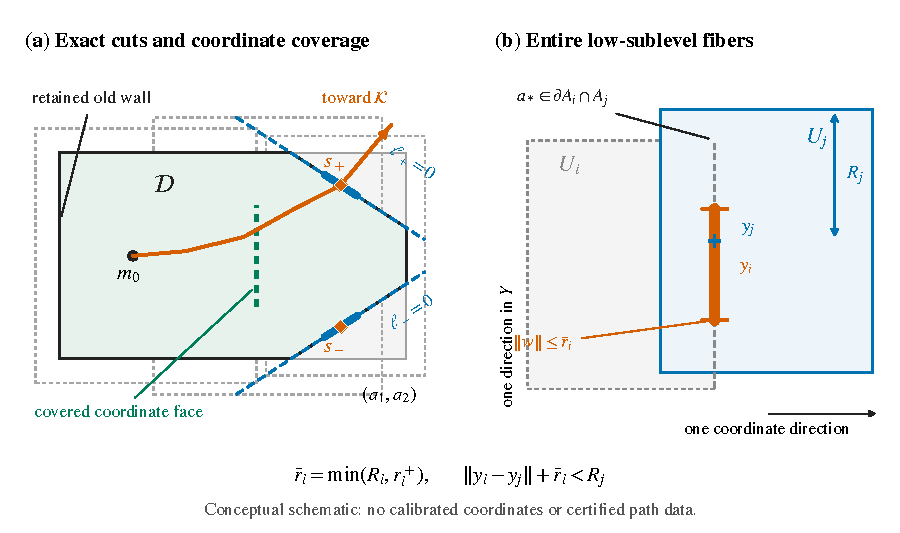
\includegraphics[width=\linewidth]{figures/certificate_geometry.pdf}
\caption{Conceptual certificate geometry; positions and proportions are
not numerical atlas data or a computed orbit. (a) Reaction coordinates,
with transverse fibers suppressed. The exact cuts pass through $s_\pm$;
thick blue segments depict local cap sections. A covered coordinate face
is internal, while a retained old wall needs an energy bound. The orange
line sketches the upper construction through $s_+$. (b) One coordinate
direction and one illustrative direction in $Y$. The entire permitted
low-sublevel fiber ball must lie strictly inside the neighboring chart,
with the complete coordinate cell inside $A_j$. The displayed Hilbert-norm
inequality, rather than overlap in this drawn slice, certifies inclusion
in every transverse direction.}
\label{fig:certificate-geometry}
% ALT TEXT: Two conceptual panels show the separating atlas. The left
% panel has overlapping coordinate rectangles, a minimum, two exact cuts
% through the saddles, a covered coordinate face, a retained outer wall,
% and an illustrative upper path. The right panel shows the complete
% allowed low-energy transverse interval inside a neighboring fiber ball.
% This interval is only a slice of the infinite-dimensional ball; the
% displayed norm inequality certifies full inclusion. No coordinates in
% the figure are calibrated certificate data.
\end{figure}

\Cref{fig:certificate-geometry} separates the local cap and chart-coverage
obligations. Because each normal lies in $\operatorname{ran}Q$, its exact
cut is constant along the $Y$ fibers. The cap bounds the fiber minimizer;
strong convexity then controls all other fiber points. Coverage of a
coordinate face instead uses inclusion of its whole possible low-energy
fiber ball, as quantified below.

For clarity, we describe the finite boundary tests. Let $h$ be the exact
level to be certified and $\overline h\ge h-e_{\rm ref}$ a verified
upper enclosure of its relative energy. Subdivide complete closed faces and intersections, including
their edges and corners. Each retained cell receives one of the
following witnesses.
\begin{enumerate}
\item A radial wall of chart $i$ passes if
\begin{equation}\label{eq:cert-radial-test}
 V_i^- -\beta_iR_i+\tfrac12\mu_iR_i^2\ge \overline h.
\end{equation}
\item Any full-fiber piece passes directly if
$V_i^--\beta_i^2/(2\mu_i)\ge \overline h$.
Otherwise put
\[
 \Delta_i=\beta_i^2+2\mu_i(\overline h-V_i^-),\qquad
 r_i^+=\frac{\beta_i+\sqrt{\Delta_i}}{\mu_i}
\]
when $\Delta_i\ge0$. A negative $\Delta_i$ excludes the sublevel.
Every point with $\E<h$ has $\nrm{w}<r_i^+$. A coordinate-face cell
is therefore internal if a chart $j$ contains its complete coordinate
cell strictly and
\begin{equation}\label{eq:cert-overlap-test}
 \nrm{y_i-y_j}+\min(R_i,r_i^+)<R_j.
\end{equation}
The stronger full-ball test replaces the minimum by $R_i$.
To prove that a point is internal to $D_0$, the coordinate cell must also
lie in $A_0$. Chart overlap alone cannot make a point on the outer
coordinate boundary internal to $D_0$.
\item A new exact-plane face passes by
\cref{lem:cert-fiber}, uniformly over its intersection with the closed
chart, coordinate region, and other cuts. Computations may overcover
the plane by the interval strip from \eqref{eq:cert-adjoint-offset}.
\item Near a cap, a retained outer boundary or seam can instead use
the following scalar cone bound. If
$H_s[r,r]\ge-A$ and
$\nrm{P_{r^\perp}H_sr}\le\kappa_r$, write
$\theta-s=tr+v$, $v\perp r$. Given
$|t|\le T$, $\nrm{v}\in[y_-,y_+]$ and
$\nrm{\theta-s}\le H_0$, set
\[
 p=\frac\mu2-\frac{\Lambda H_0}{6}>0,\quad
 q_c=\frac A2+\frac{\Lambda H_0}{6},\quad
 y_* =\operatorname{clamp}\left(\frac{\kappa_rT}{2p},y_-,y_+\right).
\]
Then the test
\begin{equation}\label{eq:cert-cone-test}
 p y_*^2-\kappa_rT y_*-q_cT^2\ge0
\end{equation}
implies $\E(\theta)\ge\E(s)$ throughout the piece. Indeed Taylor's
lower bound is
$\mu\nrm{v}^2/2-\kappa_r|t|\nrm{v}-At^2/2
-\Lambda(t^2+\nrm{v}^2)^{3/2}/6$; replacing the last square root by
$H_0$ leaves the displayed quadratic minimum.
\end{enumerate}

All quantities in these tests have interval enclosures obtained from
Gram matrices, finite loads, and the specified analytic remainders.
A boundary ledger records a complete finite closed cover and the test
used on each cell. Pairwise intersections of chart balls, a mesh of
boundary samples, or a list omitting tangencies do not establish
coverage. In particular the outer coordinate circle is checked as a
continuum. The ledger does not assert that a failed test exhibits an
actual lower-energy escape.

To make retention by the exact saddle cuts explicit, write
\[
 H_{\rm cl}=\bigcap_j\{\ell_j\le0\},\qquad
 H_{\rm op}=\bigcap_j\{\ell_j<0\},\qquad D=D_0\cap H_{\rm op}.
\]
For each closed old-wall cell $C_\alpha$, the retained set is
$C_\alpha\cap H_{\rm cl}$. The set-level obligation is
\[
 \theta\in C_\alpha\cap H_{\rm cl},\quad\E(\theta)<h
       \quad\Longrightarrow\quad\theta\in D_0.
\]
An energy bound proves this implication vacuously; a full-fiber overlap
witness proves it by strict inclusion in $D_0$. A cell may be discarded
by cuts after verifying $C_\alpha\cap H_{\rm cl}=\varnothing$.
Strict positivity of one cut throughout the cell is sufficient but not
necessary: a rigorous joint infeasibility test may also establish this.
Equality at a cut is retained whenever all other closed inequalities
hold. Exclusion from $H_{\rm op}$ alone does not justify discarding a
tangency or an old-wall/new-plane intersection.

Membership and target exclusion are additional finite tests. The entire
minimum enclosure must lie strictly inside a chart, the coordinate
region, and every retained halfspace. A useful sufficient exclusion is
\begin{equation}\label{eq:cert-vacuum-exclusion}
 \sup_{\theta\in\overline D_0}\nrm{\theta-m}<2,
\end{equation}
when $m$ has a certified charged plaquette. The four principal increments
on that plaquette imply $\E(m)\ge2$. For every $k\in\K$,
$\E(m)=\E(m-k)\le\nrm{m-k}^2/2$, so
$\operatorname{dist}_\X(m,\K)\ge2$.
The supremum in \eqref{eq:cert-vacuum-exclusion} is bounded using the
finite coordinate region, $G$, the chart centers and radii, and the
minimum enclosure. Alternatively one may certify charge preservation
throughout the closed atlas. Discreteness of $\K$ alone does not locate
the atlas relative to all its nonzero lifts.

\subsection{Upper paths attached to exact critical points}

For explicit consecutive nodes $u_j,u_{j+1}\in\X$, the global bound
$\nrm{H_\theta}\le1$ gives
\begin{equation}\label{eq:cert-segment-test}
 \max_{0\le t\le1}\E((1-t)u_j+tu_{j+1})
 \le\max\{\E(u_j),\E(u_{j+1})\}
             +\tfrac18\nrm{u_{j+1}-u_j}^2.
\end{equation}
This checks the entire time segment. The nodes use coherent real lifts;
independent choices of principal phases at successive times do not
automatically define an $\X$-continuous path.

\begin{lemma}[Stationary-endpoint attachment]\label{lem:cert-hermite}
Let $s$ be exact and stationary, $\nrm{s-\widehat s}\le\rho_s$, and
$|\E(s)-\E(\widehat s)|\le\varepsilon_s$. For an explicit node $c$,
suppose $d_c\ge\nrm{c-\widehat s}$ and
$\Delta_c^+\ge\E(c)-\E(\widehat s)$. If
\begin{equation}\label{eq:cert-hermite-test}
 \Delta_c^++\varepsilon_s+\frac\Lambda6(d_c+\rho_s)^3<0,
\end{equation}
the segment from $s$ to $c$, except at $s$, has energy strictly below
$\E(s)$.
\end{lemma}
\begin{proof}
For $g(t)=\E(s+t(c-s))$, one has $g'(0)=0$ and
$|g'''|\le\Lambda(d_c+\rho_s)^3$. Stationary-endpoint Hermite
interpolation yields
\[
 g(t)\le(1-t^2)\E(s)+t^2\E(c)
       +\frac\Lambda6(d_c+\rho_s)^3t^2(1-t).
\]
The test makes the difference from $\E(s)$ strictly negative for $t>0$.
\end{proof}

Thus no constant energy penalty proportional to $\rho_s^2$ is paid near
the saddle. Two attachment nodes enter opposite local descending sides
if their $q$-coordinates relative to $\widehat s$ have opposite signs
and absolute values greater than $\rho_s$. The positive transverse
block and negative Schur complement identify the two local strict
sublevel components. These are variational attachments, not validated
heteroclinic orbits; rigorous transition-path validation has its own
antecedents and additional obligations \cite{Breden2019}.

The minimum is attached to its candidate by the convex bridge from
\cref{lem:cert-newton}. Polygonal arms strictly below $\E(s)$ and two
tests \eqref{eq:cert-hermite-test} then connect that exact minimum through
$s$ to a terminal configuration. To reach the physical target, certify
zero charge on every terminal plaquette, including the analytic
exterior. If $\beta_e\in(-\pi,\pi]$ are its principal increments, then
$(D_e\theta-\beta_e)/(2\pi)$ is a curl-free integer bond field of finite
support. Integrating it gives a compact integer function $n$, after
subtracting its exterior constant. Hence
$\theta=2\pi n+\eta$ with $D\eta=\beta$, and
\begin{equation}\label{eq:cert-terminal-path}
 \theta(t)=2\pi n+(1-t)\eta
\end{equation}
has nonincreasing energy and ends in $\K$. The finite support follows
because a nonzero integer slip requires $|D_e\theta|\ge\pi$, and
$D\theta\in\ell^2$. Summability and domination justify continuity and
monotonicity of the infinite sum. A finite core check discharges this
condition only together with exterior branch and interface checks.
The terminal real lift need not be zero; a claim about that particular
representative requires the additional verification $n=0$.

\subsection{Global closure and reusable conditions}

\begin{theorem}[A posteriori global-barrier certificate]\label{thm:certificate}
Suppose the preceding tests validate a minimum $m$ and finitely many
index-one saddles $s_1,\ldots,s_J$. For each saddle choose a cap normal
$r_j\in\operatorname{ran}Q$ satisfying
\cref{lem:cert-cap}, and write
$\ell_j(\theta)=\inner{r_j}{\theta-s_j}$.
Fix a distinguished saddle $s_0$ and put $h=\E(s_0)$. Assume the finite
input certificate verifies the following conditions.
\begin{enumerate}
\item The exact minimum enclosure is strictly inside
$D=D_0\cap\bigcap_j\{\ell_j<0\}$, and
$\overline D_0\cap\K=\varnothing$.
\item A complete closed-cell ledger for every retained old radial,
exposed coordinate, and outer-coordinate boundary piece verifies
\eqref{eq:cert-radial-test}, the direct full-fiber bound,
\eqref{eq:cert-overlap-test}, or \eqref{eq:cert-cone-test} at level $h$.
Cells removed by another cut need not pass an energy test; their removal
must itself be verified on the complete closed cell relative to
$H_{\rm cl}$. Each retained point of energy below $h$ must be certified
strictly internal to $D_0$ by a valid coverage witness. All intersections,
edges, corners, and tangencies are included.
\item Every new face
\[
 \{\theta\in\overline D_0:\ell_j(\theta)=0,
                         \ \ell_k(\theta)\le0\ (k\ne j)\}
\]
is covered by \eqref{eq:cert-cap-lifting} and
\cref{lem:cert-fiber}, or a direct energy bound at level $h$.
For every cap used at its own saddle level, $\E(s_j)\ge h$ is certified.
\item The segment, stationary-endpoint, minimum-bridge, and terminal-lift
tests construct a path from $m$ to $\K$ with maximum $h$ through $s_0$.
\end{enumerate}
Then, over all continuous strong-$\X$ paths to the physical uniform
states,
\begin{equation}\label{eq:cert-global-identity}
 \inf_{\substack{\gamma\in C([0,1];\X)\\
        \gamma(0)=m,\ \gamma(1)\in\K}}
 \max_t\bigl(\E(\gamma(t))-\E(m)\bigr)
       =h-\E(m).
\end{equation}
\end{theorem}
\begin{proof}
The earlier tests establish exact critical points, the full-space
positive complements, and the exact cap inequalities. For a finite
union, $\partial(\bigcup_i U_i)\subset\bigcup_i\partial U_i$.
After intersecting with $a^{-1}(A_0)$ and the saddle halfspaces,
\[
 \partial D\subset
 (\partial D_0\cap H_{\rm cl})\ \cup\
 \bigcup_j(D_0\cap H_{\rm cl}\cap\{\ell_j=0\}).
\]
Indeed, every boundary point lies in $\overline D_0\cap H_{\rm cl}$;
if it is in $D_0$ and every cut is strict, it is an interior point of
$D$, a contradiction. Thus every boundary point belongs to a retained
old wall or a new plane face, including their intersections. On a coordinate wall the overlap test
places every hypothetical point below $h$ strictly inside another
chart and inside $a^{-1}(A_0)$, so it cannot belong to this boundary. All other ledger witnesses
give energy at least $h$. Hence $\E\ge h$ throughout $\partial D$.
The domain is open, contains $m$, and excludes every endpoint in $\K$.
Every admissible path has a first exit and crosses $\partial D$;
its maximum is therefore at least $h$. The validated upper path gives
the reverse inequality. No compactness of $\partial D$, attainment of
the path infimum, or invariant reduced manifold is assumed.
\end{proof}

The energy ordering in the third condition is a real obligation.
An exact symmetry preserving the energy and compatible with uniqueness
of the validated root can prove equality between reflected saddles.
Overlapping numerical energy intervals alone cannot do so.

\begin{corollary}[Several competing saddles]\label{cor:cert-competing}
If an upper path is certified through each $s_j$, and every retained
old wall is bounded below by $\min_j\E(s_j)$, then the same construction
gives barrier $\min_j\E(s_j)-\E(m)$.
\end{corollary}
\begin{proof}
Each cap is bounded below by its own saddle energy and thus by the
finite minimum. Choose a saddle attaining that minimum for the upper
path. The proof of \cref{thm:certificate} applies without determining in advance
which saddle attains the minimum.
\end{proof}

For ledger computations a direct bound by $\min_j\overline h_j$ suffices, where
$\overline h_j\ge\E(s_j)-e_{\rm ref}$ are verified relative-energy bounds. A change of
dominant mechanism requires an additional certified ordering or crossing
argument; uncertainty overlap is not evidence of a crossing. Reuse of
the theorem means verifying the same types of obligations on new data.
It does not retain old residuals, deficient-bond sets, matrix margins,
or boundary coverage automatically when the configuration changes.

\section{A certified annihilation mechanism at separation twelve}\label{sec:instance}

We now instantiate \cref{thm:certificate}. All intervals in this section are outward enclosures; the displayed decimal bounds are deliberately rounded away from the certified values. The two candidate states are stored as compact dyadic corrections to the same analytic neutral reference. Every binary floating-point input is interpreted as its exact dyadic value, rather than as an unspecified approximation. Exterior reference estimates and the core--exterior interface terms are included in the verification.

\begin{theorem}[Global dipole annihilation barrier]\label{thm:instance}
In the normalization of \cref{eq:energy-space}, there exist an exact critical state $m_0\in\X$ and two distinct exact critical states $s_\pm\in\X$ with the following properties.
The state $m_0$ has charge $+1$ at $(0,0)$, charge $-1$ at $(12,0)$, and no other charged plaquettes. It is a strict local minimum. The states $s_\pm$ are asymmetric index-one saddles interchanged by an exact lattice reflection, and $\E(s_+)=\E(s_-)=h$. At all three states the Riesz Hessian is invertible with spectral distance from zero greater than $57/1000$.

There is a bounded open set $\mathcal D\subset\X$ such that
\begin{equation}\label{eq:separator-instance}
 m_0\in\mathcal D,\qquad
 \overline{\mathcal D}\cap\K=\varnothing,\qquad
 \E(\theta)\ge h\quad(\theta\in\partial\mathcal D).
\end{equation}
There is a continuous path $\Gamma_0$ from $m_0$ to $\K$, passing through $s_+$, with $\max_t\E(\Gamma_0(t))=h$. Thus \cref{eq:intro-barrier} holds for all admissible paths of \cref{eq:barrier}, without restrictions on symmetry, extra defects, or transverse perturbations.
\end{theorem}

\begin{proof}
The frozen data and freshly evaluated inequalities verify the hypotheses of \cref{thm:certificate}. The verification has three stages. First, full dual residual bounds and signed-bond coercivity certify the minimum and the index-one saddle near their proposals. Reflection produces the second saddle with exactly equal energy; overlapping numerical energy intervals are not used to infer equality. Second, a 109-chart atlas with two reaction coordinates bounds every retained boundary wall and every exact saddle cutting plane. All transverse directions are retained as Hilbert-space fibers. Third, the validated upper construction attaches its polygonal arms to the exact saddle and to an integer phase lift at the endpoint.

The ledger includes all 436 coordinate faces, radial walls, coordinate-domain boundary portions, and the two cap planes. Five enlarged charts close the remaining plane intersections. The projected-normal and adjoint checks use the exact correction uncertainty, so the planes are not centered at the numerical saddle. The minimum-membership and vacuum-exclusion checks establish \cref{eq:separator-instance}. The global conclusion now follows from \cref{thm:certificate}. The rational energy-difference enclosures give the strict bracket in \cref{eq:intro-barrier}. Numerical margins and the executed supervisor are recorded below and in the supplementary record.
\end{proof}

\subsection{Margins and certificate geometry}

\begin{table}[t]
\caption{Verified inputs and conservative consequences. Candidate quantities are not substituted for exact-state conclusions. The original execution used the valid coarser Hessian Lipschitz constant $1$ for the correction deductions shown here.}
\label{tab:margins}
\centering\small
\begin{tabular}{@{}L{.57\linewidth}L{.34\linewidth}@{}}\toprule
Quantity & Bound\\\midrule
Minimum candidate coercivity & $>0.075672$\\
Minimum correction radius $\rho_m$ & $<0.01742120$\\
Exact minimum coercivity & $>0.05825080$\\
Saddle candidate negative Rayleigh value & $<-0.06992563$\\
Saddle candidate complementary coercivity & $>0.07195499$\\
Saddle correction radius $\rho_s$ & $<0.01282494$\\
Exact saddle inverse-gap lower bound & $>0.05710069$\\
Common exact-state gap $\sigma$ & $57/1000$\\
Exact minimum principal-branch margin & $>1.1$\\
Exact cap transverse coercivity (safe value) & $1/25$\\
Exact cap radius & $33/200$\\
Reaction-coordinate disk radius & $6599/10000$\\
Atlas charts / coordinate faces & $109$ / $436$\\\bottomrule
\end{tabular}
\end{table}

The cap parameters in \cref{tab:margins} use a different, sharper
Lipschitz bound than the conservative correction deductions.
With $\tau=71/100$ one has $2\tau^2=5041/5000>1$, hence
$\Lambda=1/\sqrt2<\tau$. Consequently the safe cap values give the
entirely rational margin
\[
 k_c\ge\frac1{50}
       -\frac{71}{100}\frac{33}{1200}
       =\frac{19}{40000}>0.
\]
The cap checker enforces $R_c<3\sqrt2\mu$, consistently with this
choice. Using $\Lambda=1$ in this cap calculation with only
$\mu=1/25$ would not give a positive coefficient; its separate use
for Newton correction bounds does not require that substitution.

The indefinite Hessian test controls its complete complement and the mutual interactions of the deficient bonds. Its negative direction need not be an eigenvector. The complement estimate together with a negative Rayleigh direction gives invertibility and index one by the reflected-coercivity argument in \cref{sec:certificate}; the exact-state uncertainty is then subtracted. This distinction matters when extending finite signed-Laplacian tests to an infinite exterior.

The atlas uses a rank-two subspace $Q\R^2$, with orthogonal complement $Y$. For each coordinate cell, the lower bound on the entire transverse fiber is evaluated, not just at its center. A face whose lower bound is too low must be covered strictly by another chart, over the whole closed cell and its entire permitted low-energy transverse ball. The final cutting planes pass through $s_\pm$. On those planes the exact saddle energy cancels algebraically, permitting the boundary threshold to equal $h$ without requiring an interval comparison with a positive margin at the saddle itself.

The upper path has only two implicit critical vertices, $m_0$ and $s_+$. Every other vertex except the zero endpoint has the analytic reference plus a compact correction. Interior segments use the quadratic interpolation bound. The two attachments to $s_+$ exploit stationarity at the exact endpoint and a cubic remainder, rather than charging a constant correction error all the way to that endpoint. The terminal contraction is checked after identifying the integer lift on the full lattice. These facts are also the inputs for the path-tail estimate in \cref{sec:green}.

\subsection{Executed verification and trust boundary}

The three frozen archives contain the separator, upper connection, and exact-cap extension. The supplementary index specifies their byte lengths and SHA-256 hashes. They are mathematical inputs with source code, dyadic proposals, and exterior formulas; archived output files are not premises in the fresh run. The command executed in a clean extraction was
\begin{quote}\small
\begin{verbatim}
python3 verify_optimality.py \
  --separator-package ../xy_global_separator \
  --connection-package ../xy_global_connection \
  --output results_fresh --workers 2
\end{verbatim}
\end{quote}
The final status was \texttt{FRESH\_OPTIMAL\_ANNIHILATION\_BARRIER\_PASS}.
The new run on 21 October 2026 took 737.33 seconds using Python 3.12.14 and g++ 13.3 on x86\_64 Linux. The compilation disabled fast arithmetic transformations and floating-point contraction, and enabled rounding-sensitive compilation. The record includes the precise flags, the final certificate hash, all 548 fresh outputs and their hashes, and the integrity check of all 1,808 original archive members. The preceding execution and its resource observations are retained as dated history.

The verifier combines exact rational bookkeeping with outward floating-point enclosures and analytic tail estimates. Candidate search, proposal optimization, and basis generation are outside the supervisor; the fixed proposals must pass its checks. The default supervisor does not execute every historical attack script, the separate secondary boundary implementation, or the separate heteroclinic extension. We therefore base \cref{thm:instance} on the global variational certificate, not on an unreported fresh heteroclinic calculation.

A further audit on 21 October 2026 rebuilt the standalone separator
from its unchanged pinned sources: all 109 local charts and all boundary
checks passed. Its 330 directly comparable scientific outputs agreed
byte for byte with the archived record. A separately coded exact-dyadic
Laplacian calculation verified all 715 geometric interval inclusions
and three scalar maxima. The later complete execution described above
also rebuilt the connection and optimality assembly from unchanged sources.

Separate instrumented copies check finite ordered interval endpoints and
the actual decimal exports against exact binary values. These fixed-data
diagnostics and independent rational geometry checks are documented in
the supplement. They do not repair the original congruence helper's
generic failure to reject an injected NaN; no such failure was found
in the protected fixed-data runs. Appendix~\ref{app:reflected-residual}
derives the residual's zero mean and explicit exterior constants.

The supported reproduction target is little-endian IEEE binary64 input
with round-to-nearest arithmetic and a \texttt{long double} significand
of exactly 64 bits. The companion environment preflight checks this
target before a new global run. The frozen extension prints its consumed
interval endpoints with an additional outward step and 30 decimal digits;
the significance of that padding is tied to this arithmetic format.
The source guard allowing at least 64 bits is not a validation of all wider
formats. In particular, portability to a 113-bit significand requires a
separate serialization analysis or a revised exact-output interface.

Reproduction with the same software tests that the distributed inputs and source produce the asserted output. It does not independently validate the underlying interval implementation or formalize the analytic reductions. The proof in \cref{sec:certificate}, the full frozen sources, and the supplementary command and integrity record expose those dependencies for examination. The new rational checkers for \cref{sec:green,sec:robustness} verify their arithmetic implications; they do not rerun this global supervisor or replace the analytic proofs.

\section{An explicit Green estimate on the certificate's energy scale}
\label{sec:green}

The exterior estimate needed by the certificate concerns the energy norm,
including at an index-one saddle.  Decay of finite-energy critical fields
under stability of the homogeneous lattice is already established in
\cite[Theorem~2.3]{Ehrlacher2016}; that regularity theorem does not require
strong stability of the critical point.  Higher-order far-field conditions
and their approximation properties have also been developed for crystalline
defects \cite{Braun2025,Wei2026}.  Our purpose here is quantitative: we give
an elementary bound with explicit constants, connect it to the same
projections used by the certificate, and retain uniformity under the
distributed coupling perturbations considered in this article.

Identify integer coordinates with physical vertices by
$x\mapsto(6+x_1+\tfrac12,x_2+\tfrac12)$, and use canonical bonds
$(x,i)=(x,x+e_i)$, where $x\in\Z^2$ and $i\in\{1,2\}$.
The point $x$ is the \emph{anchor} of the bond.  Write
$D_i\theta(x)=\theta(x+e_i)-\theta(x)$ and
$\mathcal H=\ell^2(\Z^2\times\{1,2\})$.  Each unoriented bond is counted
once.  Let $\mathsf P:\mathcal H\to D(\X)$ be the orthogonal gradient
projection.  The range is closed because $D:\X\to\mathcal H$ is an
isometry onto its image.

\begin{lemma}[A numerical kernel bound]
\label{lem:green-kernel}
The convolution kernel of $\mathsf P$ satisfies
\begin{equation}
 |\mathsf P_{ij}(z)|\le\frac{8}{(1+\nrm{z}_\infty)^2},
 \qquad z\in\Z^2,\quad i,j\in\{1,2\}.
 \label{eq:green-kernel}
\end{equation}
For each source orientation $j$ and each integer $\rho\ge1$,
\begin{equation}
 \left(\sum_{\nrm{z}_\infty\ge\rho}\sum_{i=1}^2
       |\mathsf P_{ij}(z)|^2\right)^{1/2}
 \le\frac{16\sqrt2}{\rho}.
 \label{eq:green-column}
\end{equation}
Moreover, the norm of evaluation on any bond is exactly
\begin{equation}
 |D_e v|\le 2^{-1/2}\nrm{v}_\X,
 \qquad \nrm{D_e}_{\X^*}=2^{-1/2}.
 \label{eq:edge-evaluation}
\end{equation}
\end{lemma}

\begin{proof}
For $d_i(k)=\exp(\mathrm i k_i)-1$, the Fourier symbol is
$d_i\overline{d_j}/(|d_1|^2+|d_2|^2)$ away from the origin.
Integrating one coordinate exactly gives
$|\mathsf P_{ij}(z)|\le\pi/(2r^2)<2/r^2$ for
$r=\nrm{z}_\infty\ge1$, with the shifts of the mixed coefficients
included.  Appendix~\ref{app:green-kernel} supplies that calculation.
Since $r+1\le2r$, it proves \eqref{eq:green-kernel}; at $z=0$ the bounded
Fourier multiplier gives $|\mathsf P_{ij}(0)|\le1$.
There are $8r$ anchors on the shell of radius $r\ge1$.  Therefore
\[
 \sum_{\nrm{z}_\infty\ge\rho,i}|\mathsf P_{ij}(z)|^2
 \le1024\sum_{r\ge\rho}\frac{r}{(1+r)^4}
 \le1024\int_\rho^\infty t^{-3}\,dt
 =\frac{512}{\rho^2}.
\]
This proves \eqref{eq:green-column}, including both target orientations.
Finally $\mathsf P_{11}(0)=\mathsf P_{22}(0)=1/2$: the two diagonal
symbols sum to one almost everywhere and are exchanged by coordinate
symmetry.  The squared norm of a coordinate functional restricted to
$D(\X)$ is $\mathsf P_{ii}(0)$.  This proves
\eqref{eq:edge-evaluation} by translation invariance.
\end{proof}

\subsection{A stationary source and a dyadic tail inequality}

The following statement also permits noncompact perturbations of the
couplings.  Set
\[
 E_b(\theta)=\sum_e(1+b_e)(1-\cos D_e\theta),
 \qquad b\in\ell^1(\mathcal E),
\]
so that $E_0=\E$.  For an integer anchor radius $R\ge1$, define
\begin{equation}
 T_\theta(R)=
 \left(\sum_{\nrm{x}_\infty\ge R}\sum_{i=1}^2
          |D_i\theta(x)|^2\right)^{1/2}.
 \label{eq:anchor-tail}
\end{equation}

\begin{theorem}[An effective $R^{-1}$ tail]
\label{thm:green}
Let $DE_b(\theta)=0$ in $\X^*$, $\nrm{\theta}_\X\le M$, and suppose
that an integer $R_*\ge1$ and a number $\eta\ge0$ satisfy
\[
 |D_i\theta(x)|\le\eta
 \quad\text{whenever }\nrm{x}_\infty\ge R_*.
\]
Put
\begin{align}
 q_e&=D_e\theta-(1+b_e)\sin(D_e\theta),
 &Q&=\nrm{q}_{\ell^1},\notag\\
 a&=\frac{\eta^2}{6}+\nrm{b}_{\ell^\infty},
 &R_n&=2^nR_*.
 \label{eq:green-source}
\end{align}
If $2a<1$, then
\begin{equation}
 Q\le\frac{M^3}{6}+\nrm{b}_{\ell^1},\qquad
 T_\theta(R_n)\le\frac{A}{R_n}\quad(n\ge0),
 \label{eq:green-tail}
\end{equation}
where
\begin{equation}
 A=\max\left\{R_*T_\theta(R_*),
       \frac{32\sqrt2 Q}{1-2a}\right\}.
 \label{eq:green-A}
\end{equation}
For an arbitrary real radius $R\ge R_*$, the bound
$T_\theta(R)\le2A/R$ holds.
\end{theorem}

\begin{proof}
The global inequality $|t-\sin t|\le|t|^3/6$ and
$\ell^2\subset\ell^3$ give
$\nrm{D\theta-\sin(D\theta)}_{\ell^1}\le M^3/6$.
Also $\nrm{b\sin(D\theta)}_{\ell^1}\le\nrm{b}_{\ell^1}$.
Thus $q\in\ell^1\cap\mathcal H$ and the asserted bound for $Q$ holds.
Criticality states that $(1+b)\sin(D\theta)$ is orthogonal to every
gradient.  Since $D\theta\in D(\X)$,
\begin{equation}
 D\theta=\mathsf Pq.
 \label{eq:green-representation}
\end{equation}
This uses the Riesz formulation in $\X$; it assumes no bounded inverse
of the vertex Laplacian on $\ell^2(\Z^2)$.

The role of force balance in dislocation far-field estimates is examined
in the recent preprint \cite{BraunHudson2026}. Here
\eqref{eq:green-representation} follows directly from stationarity and
the closed gradient projection. If it is rewritten as the vertex equation
$D^*D\theta=D^*q$, then $q\in\ell^1$ implies $D^*q\in\ell^1$ and
$\sum_x(D^*q)(x)=0$: absolute convergence permits pairing the two
opposite endpoint contributions of every bond. Thus this cancellation
is proved from the source representation, rather than inferred from
far-field decay.

For an even integer $R\ge2R_*$, split $q=q_{\rm in}+q_{\rm out}$ at
the anchor radius $R/2$, assigning anchors of radius $R/2$ to the exterior.
For a target anchor of radius at least $R$ and a source anchor of radius
less than $R/2$, their separation is at least $R/2$.
Minkowski's inequality and \eqref{eq:green-column} yield
\[
 \nrm{\mathbf1_{\{\nrm{x}_\infty\ge R\}}
              \mathsf Pq_{\rm in}}_{\mathcal H}
 \le\frac{32\sqrt2}{R}\nrm{q_{\rm in}}_{\ell^1}
 \le\frac{32\sqrt2 Q}{R}.
\]
On the exterior source set,
\[
 |q_e|\le\frac{|D_e\theta|^3}{6}
          +|b_e|\,|\sin D_e\theta|
 \le a|D_e\theta|.
\]
The contraction property of $\mathsf P$ therefore gives
\begin{equation}
 T_\theta(R)\le\frac{32\sqrt2 Q}{R}+aT_\theta(R/2).
 \label{eq:green-recurrence}
\end{equation}
For $A_n=R_nT_\theta(R_n)$ this is
$A_n\le32\sqrt2 Q+2aA_{n-1}$.  The interval $[0,A]$, with $A$ as
in \eqref{eq:green-A}, is invariant under this scalar inequality.
Induction proves \eqref{eq:green-tail}.  More explicitly,
\[
 A_n\le(2a)^nA_0+
       \frac{32\sqrt2 Q\,[1-(2a)^n]}{1-2a}.
\]
If $R_n\le R<R_{n+1}$, monotonicity gives
$T_\theta(R)\le A/R_n\le2A/R$.
\end{proof}

\begin{remark}
No support or moment condition on $b$ is used.  The exterior perturbation
is $b_e\sin(D_e\theta)$, which is controlled \emph{multiplicatively} by
$D_e\theta$.  Replacing it by an independent additive source would lose
this property and would require additional tail information.
\end{remark}

\subsection{The same compact projections and the upper path}

Let $\X_S$ contain the configurations with a representative zero outside
the integer vertex box $\Lambda_S=[-S,S]^2$, and let
$\Pi_S:\X\to\X_S$ be the energy-orthogonal projection.
The distinction between anchor and endpoint radii is needed when these
projections are compared with stored exterior bounds.

\begin{lemma}[A cutoff on the common energy scale]
\label{lem:green-projection}
For every $\theta\in\X$ and integer $R\ge1$,
\begin{equation}
 \nrm{(I-\Pi_{2R})\theta}_\X
 \le\sqrt{227}
 \left(\sum_{\min(\nrm{x}_\infty,\nrm{y}_\infty)\ge R}
                   |D_{\{x,y\}}\theta|^2\right)^{1/2}
 \le\sqrt{227}\,T_\theta(R).
 \label{eq:green-projection}
\end{equation}
In particular, under Theorem~\ref{thm:green}, the left side at $R=R_n$
is at most $\sqrt{227}A/R_n<16A/R_n$.
\end{lemma}

\begin{proof}
On $\mathcal A_R=\{x:R\le\nrm{x}_\infty\le2R\}$, the discrete
Poincar\'e inequality has constant $(225/4)R^2$
(Appendix~\ref{app:green-annulus}).  Let $c$ be the annular mean and let
$\zeta_R$ equal one up to radius $R$, zero from radius $2R$ onwards,
and interpolate linearly between them.  The compact representative
$\zeta_R(\theta-c)$ gives an admissible approximation in $\X_{2R}$.
Using the exact product identity
$D(fg)=\overline f\,Dg+\overline g\,Df$, where bars denote endpoint
averages, and
$2|\overline f|^2\le|f_x|^2+|f_y|^2$, its squared error is bounded by
\[
 2\sum_{\min(\nrm{x}_\infty,\nrm{y}_\infty)\ge R}|D_e\theta|^2
 +\frac4{R^2}\sum_{\mathcal A_R}|\theta-c|^2
 \le227\sum_{\min(\nrm{x}_\infty,\nrm{y}_\infty)\ge R}|D_e\theta|^2.
\]
An edge below this minimum-endpoint radius has zero error gradient:
integer neighboring radii differ by at most one and the cutoff is still
one at radius $R$.  Best approximation proves the first inequality.
Every edge in that tail has its canonical anchor of radius at least $R$,
which proves the second.
\end{proof}

For the homogeneous certificate, the known upper path is polygonal.
Its only implicit vertices are the exact minimum and the selected exact
saddle.  Each remaining vertex, except the zero endpoint, is $\phi_{12}$ plus a
stored compact correction. Here
\[
 \phi_{12}(x)=\arg(6+x_1+\tfrac12+\mathrm i(x_2+\tfrac12))
 -\arg(-6+x_1+\tfrac12+\mathrm i(x_2+\tfrac12)).
\]
The argument branches cancel their far-field jumps outside the segment
between the two poles.  Once $R\ge16$ and the projection box contains those supports, their
projection errors obey the direct dipolar bound $480/R$, proved in
Appendix~\ref{app:green-inputs}.
Consequently, if $A$ bounds both critical vertices in
Theorem~\ref{thm:green}, linearity and convexity of the norm give
\begin{equation}
 \sup_t\nrm{(I-\Pi_{2R_n})\Gamma_0(t)}_\X
 \le\frac{C_\Gamma}{R_n},\qquad
 C_\Gamma=\max\{16A,480\}.
 \label{eq:green-path}
\end{equation}
No stationary equation is assigned to a segment between vertices.

For finite-box barriers, restrict the paths in \eqref{eq:barrier} to
$\X_S$ and the endpoints to $\K\cap\X_S$, retaining all bonds crossing
the vertex-box boundary. Denote the resulting barrier by $B_S(u)$ and
write $B_\infty=B_0$, $C_\infty(u)=\E(u)+B_0(u)$.
For a compact origin $u\in\X_{2R_n}$, suppose that its segment to $m_0$
lies below the certified level $h$, and that the separator gives
$C_\infty(u)=h$.  If $M_\Gamma$ bounds the norm on that segment and on
$\Gamma_0$, then
\begin{equation}
 0\le B_{2R_n}(u)-B_\infty(u)
 \le\frac{M_\Gamma C_\Gamma}{R_n}.
 \label{eq:green-barrier-localization}
\end{equation}
Indeed, concatenate the segment and $\Gamma_0$ and apply $\Pi_{2R_n}$.
The original upper path ends at zero: its terminal check gives
\texttt{compact\_integer\_lift\_max}=0.
Thus the origin and that endpoint are unchanged. Since
$\nrm{\nabla_\X\E(z)}_\X\le\nrm{z}_\X$ and $\Pi_{2R_n}$ is a
contraction, the energy change of each projected point is at most
$M_\Gamma$ times its projection error.  This yields the upper bound;
the inclusion of finite-box paths in the infinite path class gives the
lower bound.  Thus the comparison uses the same strong energy topology
and keeps all boundary bonds of the finite box.

\subsection{Numerical consequences and uniform perturbed tails}

The payload inequalities in Appendix~\ref{app:green-inputs} permit
$M=M_\Gamma=6007$ for the certified path and for compact origins satisfying
$\nrm u_\X\le6007$, with exterior minimum-endpoint radius $4096$, and
$\eta=9/500$.  The original upper path uses $m_0$ and $s_+$, so anchor
radius $R_*=4097$ is sufficient.  Replacing $32\sqrt2$ by $46$ and
$\sqrt{227}$ by $16$ gives the rational constants
\begin{equation}
 A\le\frac{1246352073472250000}{749919},\qquad
 M_\Gamma C_\Gamma
 \le\frac{119789390485564892000000}{749919}.
 \label{eq:green-data-constants}
\end{equation}
Exact rational arithmetic gives the following budgets for the allocation
$M_\Gamma C_\Gamma/R_n\le\varepsilon/4$:
\begin{center}
\begin{tabular}{cclc}
\hline
$\varepsilon$ & $n$ & $R_n=4097\,2^n$ & error upper bound\\
\hline
$10^{-2}$ & $54$ & $73804990693347688448$ & $<2.165\,10^{-3}$\\
$10^{-6}$ & $68$ & $1209220967519808527532032$ & $<1.321\,10^{-7}$\\
\hline
\end{tabular}
\end{center}
The actual projection box has radius $2R_n$.
These are arithmetic bounds, not newly computed barrier intervals.
They replace the thousands-of-digits radii from the weak hole-filling
estimate by $20$- and $25$-digit values of $R_n$, but still cannot be
materialized.  A full cubical covering would also retain its exponential
dependence on the finite dimension.  Useful radii require sharper
data-dependent bounds for $Q$ and $T_\theta(R_*)$ and the retained
low-dimensional reaction reduction.

The same estimate is uniform over the nearby critical families of the
robustness theorem.  For all three critical states, including the reflected
saddle, use the common values
\begin{equation}
 \nrm{b}_{\ell^1}\le\frac1{500},\quad M=6008,\quad
 \eta=\frac{41}{1000},\quad R_*=4098.
 \label{eq:green-robust-data}
\end{equation}
Here a displacement of at most $1/32$ in $\X$ changes every bond
increment by at most $1/(32\sqrt2)$, so
$0.018+1/(32\sqrt2)<0.041$.  The extra radial unit is deliberate:
the physical reflection $x_1\mapsto12-x_1$ sends integer indices
$i\mapsto-i-1$, and a reoriented horizontal bond anchor to $-i-2$.
An anchor radius of $4098$ therefore guarantees reflected minimum
endpoint radius $4096$.
With \eqref{eq:green-robust-data},
\[
 a\le\frac{13681}{6000000},\qquad
 Q\le\frac{54216288128003}{1500},\qquad
 A\le\frac{4987898507776276000}{2986319}<1.7\,10^{12}.
\]
In particular, all these exact critical states satisfy, on the common
dyadic sequence,
\begin{equation}
 T_\theta(R_n)\le\frac{1.7\,10^{12}}{R_n},\qquad
 \nrm{(I-\Pi_{2R_n})\theta}_\X
 \le\frac{2.72\,10^{13}}{R_n}.
 \label{eq:green-robust-tail}
\end{equation}
This last conclusion allows noncompact $\ell^1$ coupling perturbations.
It is a uniform mathematical tail statement; an implementation accepting
arbitrary infinite inputs still requires an effective representation of
their coefficients and the relevant membership bounds.

\section{A terminating certificate on an explicit infinite input class}
\label{sec:local-class}

The global theorem can be reused without searching for a new separator
when an input is connected to $m_0$ below its certified communication
height. This section specifies an infinite class with a quantitative
tail and a terminating enclosure procedure. It concerns the homogeneous
interaction $b=0$. It neither identifies the continued saddles in a
perturbed interaction as minimax realizers nor supplies a complete search
for arbitrary configurations.

Define the absolute communication height
\[
 c(u)=\inf_{\gamma(0)=u,\ \gamma(1)\in\K}
                  \max_{0\le t\le1}\E(\gamma(t))
      =\E(u)+B_0(u),
\]
with the path class of \cref{eq:barrier}. All norms below are in $\X$.

\begin{lemma}[Subcritical connection]\label{lem:subcritical}
Suppose $c(m)=h$, $\E(m)<h$, and a continuous path from $m$ to $u$
has maximum energy $a<h$. Then $c(u)=h$.
\end{lemma}
\begin{proof}
Concatenation with an arbitrarily near-optimal path from $m$ gives
$c(u)\le\max(a,h)=h$. If $c(u)<h$, a path from $u$ to $\K$ with
maximum strictly below $h$ exists by the definition of the infimum.
Prepending the given connection would contradict $c(m)=h$.
No compactness or attainment assertion for a new minimax is used.
\end{proof}

\begin{theorem}[Reuse on a full energy ball]\label{thm:local-class}
Let $m_0,s_+,h$ be the exact states and height in
\cref{thm:instance}, and put $r=1/20$. For every
$u\in\overline B_\X(m_0,r)$,
\begin{equation}\label{eq:class-height}
 c(u)=h,\qquad B_0(u)=h-\E(u),\qquad
 0.00442867<B_0(u)<0.00570116.
\end{equation}
These inputs have the same two plaquette charges as $m_0$ and no
additional charges. They need not themselves be stationary.
For the specified flow \eqref{eq:flow} with $b=0$, the ball is invariant
and
\begin{equation}\label{eq:class-flow}
 \nrm{u(t)-m_0}\le
 e^{-43t/2000}\nrm{u(0)-m_0}.
\end{equation}
\end{theorem}
\begin{proof}
Stationarity and $H\preceq I$ give, for $v=u-m_0$ and $0\le t\le1$,
\[
 \E(m_0+tv)\le\E(m_0)+\tfrac12t^2\nrm v^2
 \le\E(m_0)+\frac1{800}<h.
\]
The last strict inequality uses $h-\E(m_0)>0.00567867$.
\Cref{lem:subcritical} proves the height identity. The exact minimum
has coercivity greater than $57/1000$. With $\tau=71/100>\Lambda$,
throughout the ball
\begin{equation}\label{eq:class-mu}
 H(u)\succeq\left(\frac{57}{1000}-\tau r\right)I
            =\frac{43}{2000}I.
\end{equation}
Thus $\E(u)\ge\E(m_0)$, proving both barrier bounds since
$0.00567867-1/800=0.00442867$. The global principal-branch margin
at $m_0$ exceeds $1.1$, while every bond changes by at most
$r/\sqrt2<1.1$. Charges are therefore preserved along the segment.
The gradient is globally Lipschitz. Pairing the evolution with $u-m_0$
and integrating \eqref{eq:class-mu} along a segment proves invariance
of the ball and \eqref{eq:class-flow}.
\end{proof}

\subsection{Inputs with a tail imposed by their construction}

Use the integer vertex boxes $\Lambda_R$ and projections $\Pi_R$ of
\cref{sec:green}. Set $R_0=4098$, $R_n=2^nR_0$, and
$w_n=r2^{-(n+1)}$. An input program supplies a compact rational field
$q_n$ supported in $\Lambda_{R_n}$ for every requested integer $n\ge0$.
Define
\begin{equation}\label{eq:class-blocks}
 v_n=\frac{w_n}{\max\{1,\nrm{q_n}^2\}}q_n,\qquad
 v=\sum_{n=0}^{\infty}v_n,\qquad u=m_0+v.
\end{equation}
The norm squared is an exact rational full-lattice bond sum, including
all bonds crossing the support boundary. The program is required to
return a finite array for every requested $n$; no decision of totality
for arbitrary programs is asserted. Call the resulting class
$\mathcal C_{\rm loc}$. It permits arbitrary rational block shapes
and signs, without symmetry assumptions.

\begin{proposition}[Certified localization]\label{prop:class-tail}
Every input \eqref{eq:class-blocks} belongs to the ball in
\cref{thm:local-class}. Its partial sums $p_N=\sum_{n=0}^Nv_n$ satisfy
\begin{equation}\label{eq:class-tail}
 \supp p_N\subset\Lambda_{R_N},\qquad
 \nrm{v-p_N}\le r2^{-(N+1)}=\frac{rR_0}{2R_N}.
\end{equation}
In particular, with $C_*=2.72\times10^{13}$,
\begin{equation}\label{eq:class-projection}
 \nrm{(I-\Pi_{2R_N})u}\le
 \frac{C_*+rR_0/2}{R_N}.
\end{equation}
\end{proposition}
\begin{proof}
For $t\ge0$, $t/\max(1,t^2)\le1$. Hence $\nrm{v_n}\le w_n$;
the geometric series gives $\nrm v\le r$ and
\eqref{eq:class-tail}. Since $p_N\in\X_{2R_N}$, best approximation
gives the same bound for $(I-\Pi_{2R_N})v$. The critical-state bound
\eqref{eq:green-robust-tail}, applied with $b=0$ on its sequence
$R_N=4098\,2^N$, gives the remaining term in
\eqref{eq:class-projection}.
\end{proof}

The class has infinitely many independently variable spatial components.
For example, choose $q_n=a_n\delta_{(R_n,0)}$ with rational
$|a_n|\le1/2$. Then $\nrm{q_n}^2=4a_n^2\le1$, the normalization denominator
is one, and nonzero infinitely many $a_n$ give a
noncompact perturbation. The tail bounds are consequences of the input
format, rather than conclusions guessed from finite exterior samples.
Only the energy ball is proved invariant under the flow; preservation
of this particular block representation or its spatial tail rate is
not needed here and is not asserted.

\subsection{Effective critical states and finite energy enclosures}

A name for $x\in\X$ returns compact rational $x_\delta$ with
$\nrm{x-x_\delta}\le\delta$ for every positive rational $\delta$.
The analytic reference and its exterior estimates in the frozen data
provide such names for the candidate states. Finite energy-orthogonal
projections are finite Dirichlet systems; their coefficients and the
reference's arctangent values can be enclosed to any rational precision.
Their projection tails tend to zero. Compact dyadic corrections preserve
this property.

For completeness, the nonlinear correction does not require an infinite
inverse as an algorithmic primitive. Write $a_e^\sharp$ for the Riesz
representative of bond evaluation. For every compact rational field $p$,
\begin{equation}\label{eq:class-riesz}
 \nrm{a_e^\sharp-p}^2
       =\frac12-2D_ep+\nrm{Dp}_2^2.
\end{equation}
Dirichlet projections of $a_e^\sharp$ on increasing boxes are rational
and converge in $\X$, by density. Formula \eqref{eq:class-riesz}
is an exact stopping test for their error. If
$\nrm{x-x_\delta}\le\delta$, then
$\nrm{F(x)-F(x_\delta)}\le\delta$. The force at the compact field
$x_\delta$ is a finite sum of these Riesz vectors with computable sine
coefficients. For compact $z$, $H(x)z$ similarly uses only the finitely
many bonds on which $D_ez\ne0$, with computable cosine coefficients.
General effective vectors follow by $\nrm{H(x)}\le1$ and density.
Thus $F$ and the Hessian action are effective in the same norm.

Let $A=H(\widehat\theta)$ for either frozen minimum or saddle candidate.
The audited bounds imply $\nrm A\le1$ and
$\nrm{A^{-1}}\le1/\gamma$ with $\gamma=69/1000$. Spectral calculus gives
\begin{equation}\label{eq:class-inverse}
 A^{-1}f=\sum_{k=0}^{M}A(I-A^2)^kf+\mathcal R_Mf,\qquad
 \nrm{\mathcal R_Mf}\le
 \frac{(1-\gamma^2)^{M+1}}{\gamma}\nrm f.
\end{equation}
Indeed, $A$ is self-adjoint and its spectrum has modulus between
$\gamma$ and one; summing the scalar geometric identity proves the
formula also at an index-one candidate. Its finite polynomials can be
computed with the preceding oracles, and the remainder tends to zero.

The frozen Newton map $T(z)=z-A^{-1}F(\widehat\theta+z)$ is a
contraction on its original certified correction ball. Its self-map
property uses the original constants in
\cref{lem:cert-newton}; substituting a weaker common constant into that
self-map test is unnecessary. Since both correction radii are less than
$1/50$, \eqref{eq:basic-bounds} and the displayed common inverse bound
give contraction factor less than $1/4$. Exact iterates from zero
therefore have distance at most $4^{-j}/50$ from the correction.
Computing a finite composition to any prescribed additional error is
effective by \eqref{eq:class-inverse}. Thus the exact states $m_0,s_+$
have effective names. This is a constructive proof of computability,
not an assertion that the original finite-precision supervisor already
implements arbitrary-precision refinement.

\begin{theorem}[Termination on $\mathcal C_{\rm loc}$]
\label{thm:class-termination}
Given an input program of \eqref{eq:class-blocks} and a positive rational
$\varepsilon$, there is a procedure using finitely many input blocks,
finite linear systems, rational operations, and rigorously enclosed
trigonometric evaluations which returns rational $L,U$ such that
\begin{equation}\label{eq:class-enclosure}
 L\le B_0(u)\le U,\qquad U-L<\varepsilon.
\end{equation}
It uses the fixed global certificate once and does not search for a new
minimax saddle. No uniform practical complexity bound is asserted.
\end{theorem}
\begin{proof}
The preceding construction gives compact rational names for $s_+$
and, using \eqref{eq:class-tail}, for $u=m_0+v$.
Both critical states have norm at most $M_*=6008$ by the existing
common Green data. Thus $\nrm u\le M_*+r$.
For an approximation $x_\delta$ to an exact field $x$, Taylor expansion
at $x$ and $\nrm{F(x)}\le\nrm x$ give
\[
 |\E(x_\delta)-\E(x)|\le\nrm x\,\delta+\tfrac12\delta^2.
\]
Choose
\[
 \delta=\min\left\{1,
 \frac{\varepsilon}{8(2M_*+r+1)}\right\}.
\]
Compute the two names to this accuracy and enclose each finite bond
energy sum with radius at most $\varepsilon/16$, using rational Taylor
remainders for cosine. The error in the difference of the exact and
compact energies is at most
$(2M_*+r)\delta+\delta^2\le\varepsilon/8$.
Adding the two finite-sum errors gives a rational interval of radius
at most $\varepsilon/4$. Its width is at most
$\varepsilon/2<\varepsilon$. By \cref{thm:local-class} it encloses
$\E(s_+)-\E(u)=B_0(u)$. Each requested accuracy entails finitely many
blocks and oracle operations, and each refinement loop has a proven
vanishing error. This proves termination.
\end{proof}

The compact-name tolerance can be divided between the name of $m_0$
and the block tail; there is no need to materialize the very large
projection radius in \eqref{eq:class-projection}. The latter is a
separate spatial localization guarantee. The supplementary rational
checker verifies the constants, representative finite block prefixes,
and error budgets. The general critical-name and arbitrary-input
enclosure procedure above is proved, but is not advertised as an
executed general software interface. The substantive global certificate
remains \cref{thm:instance}; subcritical concatenation is its elementary
reuse principle, not an independent claim of a new universal method.

\section{Robustness under spatially inhomogeneous couplings}
\label{sec:robustness}

We now extend the single homogeneous certificate to a class of perturbed
energies. The extension preserves a positive \emph{global} annihilation
barrier and gives a uniform dynamical stability statement. It does not
identify the perturbed minimax with the height of a particular continued
saddle.

Write $m_0,s_+,s_-$ for the certified unperturbed minimum and saddles,
and put
\[
 h=\E(s_+)=\E(s_-),\qquad B_0=h-\E(m_0).
\]
We use the certified domain $\mathcal D$, whose closure misses $\K$, and the
certified upper path $\Gamma_0$ from $m_0$ to $\K$, so that
\begin{equation}
 \label{eq:robust-seed-global}
 m_0\in\mathcal D,\qquad \E|_{\partial\mathcal D}\ge h,
 \qquad \max_t\E(\Gamma_0(t))=h,
 \qquad .00567867<B_0<.00570116.
\end{equation}
All operator norms and gradients in this section refer to the Riesz
identification associated with the $\X$ inner product.

For $b\in\ell^1(\mathcal E;\R)$ define
\begin{equation}
 \label{eq:coupling-energy}
 E_b(u)=\sum_{e\in\mathcal E}(1+b_e)(1-\cos D_eu)
       =\E(u)+W_b(u).
\end{equation}
The endpoint set remains $\K$ when $1+b_e>0$. Denote by $B_b(a)$ the
annihilation barrier for $E_b$ starting from $a$: its paths are all strong
$\X$-continuous paths from $a$ to $\K$, with no prescribed charge history,
symmetry, or exterior configuration.

\begin{lemma}[Uniform differential and oscillation bounds]
\label{lem:coupling-bounds}
Let $p=\nrm{b}_{\ell^1}$. Then $W_b$ is smooth on $\X$, and
\begin{align}
 \nrm{\nabla_{\X}W_b(u)}&\le\frac{p}{\sqrt2},&
 \nrm{H_{W_b}(u)}&\le\frac p2,\label{eq:coupling-derivatives}\\
 \nrm{H_b(u)}&\le1+\frac p2,&
 \nrm{H_b(u)-H_b(v)}&\le
       \frac{1+p/2}{\sqrt2}\nrm{u-v}_{\X}.
 \label{eq:coupling-hessian}
\end{align}
Moreover, the absolutely convergent sums
\begin{equation}
 \label{eq:coupling-oscillation}
 W_-=2\sum_{b_e<0}b_e,\qquad W_+=2\sum_{b_e>0}b_e
\end{equation}
satisfy $W_-\le W_b(u)\le W_+$ for every $u\in\X$ and
$W_+-W_-=2p$.
\end{lemma}

\begin{proof}
Let $g_e$ be the Riesz representative of $D_e$. The nearest-neighbour
resistance identity gives $\nrm{g_e}_{\X}=1/\sqrt2$. Hence
\[
 \nabla_{\X}W_b(u)=\sum_e b_e\sin(D_eu)g_e,\qquad
 H_{W_b}(u)=\sum_e b_e\cos(D_eu)g_e\otimes g_e.
\]
The series converge absolutely in $\X$ and in operator norm. Their
derivatives converge locally uniformly; for derivatives of positive order
this also follows directly by summing $|b_e|\nrm{g_e}_{\X}^{j}$.
This proves smoothness and \eqref{eq:coupling-derivatives}. The unperturbed
bounds are $\nrm{H_0(u)}\le1$ and
$\nrm{H_0(u)-H_0(v)}\le\nrm{u-v}_{\X}/\sqrt2$. For the perturbation,
the Lipschitz bound on the cosine gives
\[
 \nrm{H_{W_b}(u)-H_{W_b}(v)}
 \le\sum_e|b_e|\nrm{g_e}_{\X}^3\nrm{u-v}_{\X}
 =\frac{p}{2\sqrt2}\nrm{u-v}_{\X}.
\]
This yields \eqref{eq:coupling-hessian}. Finally
for each bond the sign of $b_e$ gives
\[
 2\min(b_e,0)\le b_e(1-\cos D_eu)\le2\max(b_e,0).
\]
Absolute summability permits adding these inequalities over all bonds.
They hold for every compatible phase field, regardless of dependencies
between its increments. Thus $W_-$ and $W_+$ are lower and upper
enclosures; they need not be attainable extrema, and no independent
variation of the bond angles is required.
\end{proof}

The stationary-state certificate provides the following safe rational
information:
\begin{equation}
 \label{eq:robust-seed-gap}
 H_0(m_0)\succeq\sigma I,\qquad
 \nrm{H_0(s_\pm)^{-1}}\le\sigma^{-1},\qquad
 \operatorname{ind}H_0(s_\pm)=1,
 \qquad \sigma=\frac{57}{1000}.
\end{equation}
Indeed, the minimum's candidate coercivity exceeds $.07567$ and its
correction radius is less than $.017422$, while the saddle's candidate
inverse gap exceeds $.069925$ and its correction radius is less than
$.012825$. Subtracting the correction radii using the conservative
Hessian Lipschitz constant $1$ gives $.058248$ and $.057100$, respectively,
both greater than $\sigma$. The minimum's global principal-increment
branch margin is greater than $11/10$.

\begin{theorem}[A quantitative class of robust global barriers]
\label{thm:robustness}
Let
\[
 \delta=\frac1{500},\qquad r=\frac1{32},\qquad
 \tau=\frac{71}{100},\qquad g=\frac{541}{16000}.
\]
For every $b\in\ell^1(\mathcal E;\R)$ with $\nrm{b}_{\ell^1}\le\delta$,
the following assertions hold.
\begin{enumerate}
\item The energy $E_b$ has unique critical points $m_b,s_b^+,s_b^-$ in
the closed radius-$r$ balls about $m_0,s_+,s_-$, respectively.
These branches depend smoothly on $b$. The minimum satisfies
$H_b(m_b)\succeq gI$; each saddle has index one and inverse norm at most
$g^{-1}$. The two saddle branches remain distinct.
\item The minimum $m_b$ has precisely the original charges $+1$ and $-1$
at $(0,0)$ and $(12,0)$ and belongs to $\mathcal D$.
\item Its global annihilation barrier satisfies
\begin{equation}
 \label{eq:robust-barrier}
 \big|B_b(m_b)-B_0\big|\le2\nrm{b}_{\ell^1}.
\end{equation}
In particular, throughout this coupling class,
\begin{equation}
 \label{eq:robust-barrier-numeric}
 .00167867<B_b(m_b)<.00970116.
\end{equation}
\end{enumerate}
\end{theorem}

\begin{proof}
Since $\tau^2>1/2$, it is a rational upper bound for $1/\sqrt2$.
Fix an unperturbed critical point $z$ among the three certified states.
Taylor expansion gives
\[
 \nabla_{\X}\E(z+v)=H_0(z)v+N_z(v),\qquad
 \nrm{N_z(v)}\le\frac\tau2\nrm{v}_{\X}^2.
\]
On the radius-$r$ ball, $N_z$ has Lipschitz constant at most $\tau r$.
The equation $\nabla_{\X}E_b(z+v)=0$ is equivalent to the fixed point
equation
\[
 v=T_{b,z}(v):=-H_0(z)^{-1}
             \big[N_z(v)+\nabla_{\X}W_b(z+v)\big].
\]
By \eqref{eq:robust-seed-gap} and
Lemma~\ref{lem:coupling-bounds}, the exact self-mapping and contraction
tests are
\begin{align}
 \tau\delta+\frac\tau2r^2
 &=\frac{45227}{25600000}
 <\frac{45600}{25600000}=\sigma r,
 \label{eq:robust-newton-map}\\
 \operatorname{Lip}(T_{b,z})
 &\le\frac{\tau r+\delta/2}{\sigma}
 =\frac{371}{912}<1.
 \label{eq:robust-newton-contraction}
\end{align}
Banach's theorem produces the unique critical point $z_b$ in this ball.
At that point,
\begin{equation}
 \label{eq:robust-operator-perturbation}
 \nrm{H_b(z_b)-H_0(z)}\le\tau r+\frac\delta2
 =\frac{371}{16000},\qquad
 \sigma-\frac{371}{16000}=g.
\end{equation}
For the minimum this gives the asserted coercivity. For a saddle,
\eqref{eq:robust-seed-gap} implies that the spectrum of its self-adjoint
Hessian misses $(-\sigma,\sigma)$. Its negative spectral space is
one-dimensional and its complementary spectral space is positive.
The perturbation in \eqref{eq:robust-operator-perturbation} leaves the
quadratic form negative on the former space and positive on the latter.
Thus its index is at least one and at most one. The inverse exists by
the Neumann-series test, with norm at most
$1/(\sigma-371/16000)=g^{-1}$. This argument does not identify a
numerical saddle direction with an exact eigenvector. Smooth dependence
on the $\ell^1$ parameter follows from the smooth implicit-function
theorem and uniqueness; the strict self-mapping test keeps each root
in the interior of its ball.

For completeness, distinctness uses the recorded reaction-coordinate
enclosures. If $Q:\R^2\to\X$ is the reaction embedding and $G=Q^*Q$,
the certificate gives $\lambda_{\min}(G)>1/4$. Therefore the linear
functional consisting of the second coordinate of $G^{-1}Q^*u$ has
norm less than $2$. The candidate saddle coordinates differ by more
than $.89$ in this coordinate, and each original saddle correction has
norm less than $.013$. The exact coordinate difference is consequently
greater than $.89-4(.013)=.838$, and the original saddle distance is
greater than $.419>.4$. The continued saddle distance is then greater
than $.4-2r=27/80$.

Every bond increment changes by at most $\tau r$ between $m_0$ and
$m_b$. Its distance from the principal-branch cut remains greater than
\[
 \frac{11}{10}-\tau r=\frac{3449}{3200}>0.
\]
The straight segment crosses no branch cut, so all plaquette charges
are preserved. To establish membership in $\mathcal D$, use stationarity
of $m_0$ and the global bound $\nrm{H_0}\le1$:
\begin{equation}
 \label{eq:robust-low-bridge}
 \E\big(m_0+t(m_b-m_0)\big)
 \le\E(m_0)+\frac{r^2}{2}
 =\E(m_0)+\frac1{2048}<h,
 \qquad 0\le t\le1.
\end{equation}
Since the segment starts in $\mathcal D$, it cannot meet its boundary,
where \eqref{eq:robust-seed-global} gives $\E\ge h$. In particular
$m_b\in\mathcal D$. No inclusion of a full norm ball in $\mathcal D$
has been assumed.

It remains to prove the global estimate with the shifted origin. On
the radius-$r$ ball about $m_0$, both energies are strictly convex:
\[
 H_0\succeq(\sigma-\tau r)I>0,\qquad H_b\succeq gI>0.
\]
Stationarity at the respective minima and convexity on this ball imply
\begin{equation}
 \label{eq:robust-endpoint-energies}
 \E(m_b)\ge\E(m_0),\qquad E_b(m_b)\le E_b(m_0),\qquad
 \max_{[m_b,m_0]}E_b\le E_b(m_0).
\end{equation}
Every admissible path from $m_b$ to $\K$ must cross
$\partial\mathcal D$. Its maximal perturbed energy is at least
$h+W_-$, whereas
$E_b(m_b)\le E_b(m_0)\le\E(m_0)+W_+$. This proves
\[
 B_b(m_b)\ge B_0-(W_+-W_-).
\]
For the opposite inequality, prepend the bridge from $m_b$ to $m_0$
to $\Gamma_0$. Its energy is at most $h+W_+$: this follows on
$\Gamma_0$ from \eqref{eq:robust-seed-global}, and on the bridge
from \eqref{eq:robust-endpoint-energies}. Finally
$E_b(m_b)\ge\E(m_0)+W_-$, again by
\eqref{eq:robust-endpoint-energies}. Hence
$B_b(m_b)\le B_0+(W_+-W_-)$, which proves
\eqref{eq:robust-barrier} and \eqref{eq:robust-barrier-numeric}.
\end{proof}

\begin{corollary}[Uniform local stability for the energy-space flow]
\label{cor:flow}
For every coupling field in Theorem~\ref{thm:robustness}, the flow
\begin{equation}
 \label{eq:robust-gradient-flow}
 \dot u=-\nabla_{\X}E_b(u)
\end{equation}
is globally well posed in $\X$. If $\nrm{u(0)-m_b}_{\X}\le1/100$, then
the solution stays in that ball and
\begin{equation}
 \label{eq:robust-exponential-stability}
 \nrm{u(t)-m_b}_{\X}
 \le e^{-13t/500}\nrm{u(0)-m_b}_{\X},\qquad t\ge0.
\end{equation}
Along every solution,
$\frac{d}{dt}E_b(u)=-\nrm{\nabla_{\X}E_b(u)}_{\X}^2$.
\end{corollary}

\begin{proof}
The gradient is globally Lipschitz, with constant at most
$1+\delta/2=1001/1000$, by \eqref{eq:coupling-hessian}; the Hilbert-space
ODE therefore has a unique global solution. Moreover
\[
 \frac{1+\delta/2}{\sqrt2}<\frac{711}{1000}.
\]
Within distance $1/100$ of $m_b$, its Hessian is bounded below by
\[
 \left(\frac{541}{16000}-\frac{711}{100000}\right)I
 =\frac{10681}{400000}I\succ\frac{13}{500}I.
\]
For $w=u-m_b$, stationarity and integration along the segment from
$m_b$ to $u$ give
\[
 \frac{d}{dt}\frac{\nrm{w}_{\X}^2}{2}
 =-\inner{w}{\nabla_{\X}E_b(m_b+w)-\nabla_{\X}E_b(m_b)}
 \le-\frac{13}{500}\nrm{w}_{\X}^2.
\]
A first-exit argument makes the closed ball invariant; Gronwall's
inequality gives \eqref{eq:robust-exponential-stability}. The energy
identity follows by the chain rule.
\end{proof}

\begin{remark}[Compatibility with the effective exterior estimate]
The class above also fits the Green estimate of
Section~\ref{sec:green}, Theorem~\ref{thm:green}. For a continued critical
state $z_b$, stationarity gives
\[
 Dz_b=P_{\mathrm{grad}}q_b,\qquad
 q_b=Dz_b-(1+b)\sin(Dz_b),\qquad
 \nrm{q_b}_{\ell^1}\le\frac{\nrm{z_b}_{\X}^3}{6}
                         +\nrm{b}_{\ell^1}.
\]
Beyond the certified unperturbed exterior radius, the original increments
are bounded by $.018$. Continuation therefore gives
$|D_ez_b|\le .018+\tau/32=643/16000<.041$. On those exterior bonds,
\[
 |q_{b,e}|\le\left(\frac{.041^2}{6}+\nrm{b}_{\ell^\infty}\right)
                  |D_ez_b|
 \le\frac{13681}{6000000}|D_ez_b|,
 \qquad 2\frac{13681}{6000000}<1.
\]
Thus the required exterior source term remains absorbable uniformly
throughout the $\ell^1$ ball. In particular, a translated coupling
perturbation is not an independent additive far-field force: it retains
the factor $\sin(D_ez_b)$. No compact-support condition on $b$ is needed
for this implication.
\end{remark}

\begin{remark}[Scope of the robustness statement]
The budget $\nrm{b}_{\ell^1}\le1/500$ is a \emph{total} coupling budget.
For one modified bond it allows a relative change of $0.2\%$; it does
not allow that change independently on every bond of a growing box.
Nonzero constant rescalings of the whole lattice are outside this
$\ell^1$ class. The theorem proves neither that one of $s_b^{\pm}$
attains the perturbed minimax nor that reflection breaking selects a
different escape mechanism. Those conclusions require additional
separator and connection checks. Corollary~\ref{cor:flow} concerns the
specified $\X$ mobility, not the local $\ell^2$ gradient flow or a thermal
escape rate. The continuation and oscillation arguments are standard;
their role here is to turn the reproduced global certificate into an
explicit class of robust infinite-lattice conclusions.
\end{remark}

\section{Algorithmic scope and further certification}\label{sec:discussion}

The a posteriori theorem separates a finite verification task from the search for suitable input data. A successful certificate proves a statement about every admissible escape path in an infinite space. It need not enumerate those paths, classify all critical points, or make the separator invariant under a dynamics. Its reusable content is the collection of explicit inequalities and the requirement that their boundary ledger cover the full continuum.

\Cref{thm:class-termination} gives a terminating enclosure procedure on
$\mathcal C_{\rm loc}$ by reusing one certified communication height.
It does not search for a new saddle or certify arbitrary input states.
Its input format supplies effective tails and a subcritical connection.
The fixed global chain and the new rational arithmetic checks are
executed; the arbitrary-precision critical-name interface used in the
constructive theorem has not been implemented as a general program.

A complete algorithm for all effectively represented finite-energy XY
configurations remains an open problem. In particular, this paper does
not prove that every strict lower level admits a finite separator
recognized by its verifier. Such completeness, or a different effective
global localization theorem, would be required to justify universal
termination. Local spectral reduction alone does not provide it.

This does not give a practical search algorithm for arbitrary XY configurations. An infinite input must come with an effective representation and tail bounds; finite samples cannot certify arbitrary unseen exterior data. Even for compact inputs in the certified local class, a complete cubical search on a large truncation has exponential dimension dependence. The inverse-radius estimate improves the rigorous localization rate substantially, but its current norm majorants still yield impractical truncation sizes. The global barrier in \cref{thm:instance} was obtained from the tailored atlas and analytic exterior, not from materializing those enormous boxes.

For the perturbation family in \cref{eq:intro-perturbation}, the conclusion is stronger than persistence of an isolated finite-box root: it includes the global barrier estimate and tails in the same infinite-dimensional class. It is also weaker than a parameter-uniform identification of a transition saddle. The continued saddles are genuine index-one states, but \cref{thm:robustness} does not exclude a different route becoming cheaper under perturbation. To identify a change of mechanism, one must certify the competing upper paths and every relevant part of a common separating boundary over a parameter interval, and then prove the crossing of their exact critical heights. Two overlapping interval enclosures do not prove such a crossing.

The most direct quantitative improvement is a sharper far-field source estimate. The cubic bound $\nrm{D\theta-\sin D\theta}_1\le\nrm\theta_\X^3/6$ uses a deliberately loose global energy-norm bound. Verified core sums and cancellation or multipolar information could reduce the tail constant without changing the path-space theorem. Existing far-field expansions and higher-order boundary conditions \cite{Braun2022,Braun2025,Wei2026} suggest the right analytic tools; compatibility with an indefinite saddle and the exact global boundary remains an obligation, rather than a consequence of a stable-minimum approximation theorem.

The localization estimate has the form $C_E/R$, so an error allocation
$\varepsilon/4$ requires $R\ge4C_E/\varepsilon$. The current
$C_E\simeq1.60\times10^{17}$ explains the enormous radii: their dependence
on inverse accuracy is linear. Choosing dyadic radii does not make it
exponential. The separate exponential obstacle is a complete cubical
covering in the number of retained variables, which is of order $R^2$.
The first quantitative task is therefore to certify the actual core sum
of $|q_e|$, $q=D\theta-\sin(D\theta)$, and its exterior remainder,
replacing the coarse $M^3/6$ majorant. A further route is to extract
leading lattice multipoles before taking absolute values. For example,
with $M_j^{(q)}=\sum_yq_j(y)$ the exact identity
\[
 (\mathsf Pq)_i(x)=\sum_j\mathsf P_{ij}(x)M_j^{(q)}
 +\sum_{j,y}\bigl[\mathsf P_{ij}(x-y)-\mathsf P_{ij}(x)\bigr]q_j(y)
\]
separates the leading term. Improving the remainder requires explicit
kernel-difference bounds, controlled source moments and exterior tails,
and uniform estimates along the complete upper construction. Zero total
vortex charge does not by itself establish the needed cancellations of
this nonlinear source. In a perturbed problem these controls must also
hold in the same admitted coupling class. We have not proved a
multiphase-averaging shortcut: averaging phase representatives need not
preserve their charges or the certified energy ceiling. A materializable
method should retain an analytic exterior and the low-rank atlas, and
would still require a verified computational budget after these sharper
estimates are obtained.

\subsection*{Data and software availability}
The source repository is
\url{https://github.com/rsumoza/global_annihilation_barriers_infinite_-XY_lattice}.
The supplementary index identifies the three frozen global-verification
archives by byte count and SHA-256; they are necessary in addition to the
smaller source and checker snapshot. The planned frozen distribution is
the tagged release \texttt{siads-v7-2026-10-22} at
\url{https://github.com/rsumoza/global_annihilation_barriers_infinite_-XY_lattice/releases/tag/siads-v7-2026-10-22},
with sources in Git and the original archives attached as release assets.
The repository address has been supplied by the author; publication of
the tagged release and remote access remain to be verified. No DOI is
asserted. The tag identifies the source commit once published; its full
SHA is to be recorded in the release description and submission record.
The supplement and index accompany the initial submission. Any practical
portal restriction on the frozen material must be resolved through an
accepted submission route; external access does not automatically waive
the journal's review requirements.

\subsection*{Declarations}
OpenAI ChatGPT/Codex tools were used substantively in mathematical exploration and proof drafting, code development and execution, literature retrieval and comparison, adversarial checking, and manuscript preparation. The conceptual geometric figure is generated by explicit Python code; it is not a numerical output of the certificate. These automated checks and drafting assistance do not constitute independent external peer review or proof-assistant verification. The authors assume responsibility for all content.

\appendix\section{Details of the explicit lattice Green bound}
\label{app:green-kernel}

We justify the Fourier calculation in Lemma~\ref{lem:green-kernel} with
the canonical bond-anchor convention.  Orthogonality of a field
$f\in\mathcal H$ to $Dv$ for every compact $v$ is equivalent, after
Fourier transform, to
$\sum_i\overline{d_i}\widehat f_i=0$ almost everywhere: trigonometric
polynomials are dense and the $d_i$ are bounded.  Thus $D(\X)$ is the
pointwise span of $d=(d_1,d_2)$, apart from the irrelevant frequency zero,
and the projection symbol is
\[
 m_{ij}(k)=\frac{d_i(k)\overline{d_j(k)}}{\Lambda(k)},\qquad
 \Lambda(k)=4-2\cos k_1-2\cos k_2.
\]
This argument does not require an $\ell^2$ vertex potential for each
finite-energy gradient.  In particular, $\nrm{\mathsf P}_{\mathcal H\to
\mathcal H}=1$ and every scalar symbol is bounded by one.

Let $z=(n_1,n_2)$ and first assume
$r=|n_2|=\nrm{z}_\infty\ge1$.  For $t=k_1\ne0$, set
\[
 s=|\sin(t/2)|,\quad
 \alpha=2\operatorname{arsinh}s,\quad
 g_n(t)=\frac{e^{-\alpha|n|}}{2\sinh\alpha}.
\]
Since $\cosh\alpha=2-\cos t$, the Poisson kernel identity gives
\begin{equation}
 \frac1{2\pi}\int_{-\pi}^{\pi}
 \frac{e^{\mathrm i n y}}{4-2\cos t-2\cos y}\,dy=g_n(t).
 \label{eq:green-partial}
\end{equation}
It follows by expanding
$(\cosh\alpha-\cos y)^{-1}$ as a geometric Fourier series; all series
converge absolutely for this fixed $t\ne0$.

The partially integrated diagonal entries are
$4s^2g_{n_2}$ and $\delta_{n_2,0}-4s^2g_{n_2}$.  Since $n_2\ne0$,
their magnitudes are at most
\[
 4s^2g_{n_2}
 =\frac{s}{\sqrt{1+s^2}}e^{-\alpha r}
 \le s e^{-\alpha r}.
\]
For the $12$ entry, the partial coefficient is
$d_1[g_{n_2-1}-g_{n_2}]$; for the $21$ entry it is
$\overline{d_1}[g_{n_2+1}-g_{n_2}]$, up to the choice of Fourier sign.
For both shifts, including $r=1$,
\begin{equation}
 |g_{n_2\pm1}-g_{n_2}|
 \le\frac{e^\alpha-1}{2\sinh\alpha}e^{-\alpha r}
 =\frac{e^\alpha}{e^\alpha+1}e^{-\alpha r}
 \le e^{-\alpha r}.
 \label{eq:green-shift-bound}
\end{equation}
As $|d_1|=2s$, the two mixed entries have partial magnitude at most
$2s e^{-\alpha r}$.  Thus no unit shift of the anchor distance remains
unaccounted for.

For $0\le t\le\pi$,
$s\le t/2$, $s\ge t/\pi$, and
$\operatorname{arsinh}s\ge s/\sqrt2$.
The last inequality follows by integrating
$(1+s^2)^{-1/2}\ge1/\sqrt2$ on $[0,s]\subset[0,1]$.
Consequently
\[
 \frac1{2\pi}\int_{-\pi}^{\pi}s e^{-\alpha r}\,dt
 \le\frac1{2\pi}\int_0^\infty
      t e^{-\sqrt2 rt/\pi}\,dt
 =\frac{\pi}{4r^2}.
\]
This gives $|\mathsf P_{ij}(z)|\le\pi/(2r^2)<2/r^2$.
If $|n_1|=\nrm{z}_\infty\ge1$, exchange the axes and their orientation
labels.  At $z=0$ use the integral of the bounded scalar symbol.
The multiplier entries are bounded on a finite measure torus, so Fubini
applies directly.  The exceptional value $t=0$ has measure zero, and the
partial bounds above are integrable.  There is no appeal to an
uncontrolled logarithmically divergent vertex Green function.

\section{An annular Poincar\'e constant for the cutoff}
\label{app:green-annulus}

For $R\ge1$ integer and
$\mathcal A_R=\{x:R\le\nrm{x}_\infty\le2R\}$, we prove
\begin{equation}
 \sum_{\mathcal A_R}|u-\overline u_{\mathcal A_R}|^2
 \le\frac{225}{4}R^2\sum_{e\subset\mathcal A_R}|D_eu|^2.
 \label{eq:green-annular-poincare}
\end{equation}
For $n$ values on an interval, the variance identity and Cauchy--Schwarz
give
\[
 \sum_i|u_i-\overline u|^2
 =\frac1n\sum_{i<j}|u_i-u_j|^2
 \le\sum_{k=1}^{n-1}\frac{k(n-k)}2|u_{k+1}-u_k|^2
 \le\frac{n^2}{8}\sum_k|D u_k|^2.
\]
Decomposing the variance of an $n_1\times n_2$ rectangle into row
variances and the variance of row means, followed by Jensen's inequality,
gives the constant $\max(n_1^2,n_2^2)/8$ for its full edge energy.

Cover the annulus by its four top, right, bottom, and left strips, each
with $(4R+1)(R+1)=N$ vertices.  Adjacent strips have an overlap of
$J=(R+1)^2$ vertices.  Write $m_i$ for their means and
$V_i=\sum_{S_i}|u-m_i|^2$.  Averaging over an overlap yields
$|m_i-m_j|^2\le2(V_i+V_j)/J$.  If $c$ is the mean of the four $m_i$,
the four-cycle inequality gives
\[
 \sum_i|m_i-c|^2\le\frac12\sum_{i\sim j}|m_i-m_j|^2
 \le\frac2J\sum_i V_i.
\]
Hence
\[
 \sum_{\mathcal A_R}|u-c|^2
 \le\sum_iV_i+N\sum_i|m_i-c|^2
 \le(1+2N/J)\sum_iV_i\le9\sum_iV_i.
\]
Each edge belongs to at most two strips and $(4R+1)^2\le25R^2$.
The rectangular estimate bounds the last expression by
$9\cdot2\cdot25R^2/8$ times the annular edge energy.  Replacing $c$
by the annular mean can only decrease the variance, proving
\eqref{eq:green-annular-poincare}.

\section{Explicit dipolar and payload norm bounds}\label{app:green-inputs}

Let $L=12$ and let $\phi_{12}$ be the real reference in
\cref{sec:green}. For an index radius $r\ge16$, the distance to every
interpolated pole is at least $r-8\ge r/2$. Integrating the derivative
of the argument with respect to pole position, and then along a unit
bond, gives
\[
 |\phi_{12}(x)|\le2L/r,\qquad
 |D_e\phi_{12}|\le4L/r^2
 \quad\text{if }\min(\nrm{x}_\infty,\nrm{y}_\infty)=r.
\]
These integrations take place away from the pole segment, so they do not
introduce branch jumps. There are at most $16r+4\le20r$ bonds with
minimum endpoint radius $r$. Therefore, for integer $R\ge16$,
\[
 \sum_{\min(\nrm{x}_\infty,\nrm{y}_\infty)\ge R}
 |D_e\phi_{12}|^2
 \le320L^2\sum_{r\ge R}r^{-3}\le480L^2/R^2.
\]
For the cutoff $\zeta_R$ used in \cref{lem:green-projection}, the
annulus has $12R(R+1)\le24R^2$ vertices. Thus direct use of its product
identity gives
\[
 \nrm{(1-\zeta_R)\phi_{12}}_\X^2
 \le2(480L^2/R^2)+\frac4{R^2}
           \sum_{\mathcal A_R}|\phi_{12}|^2
 \le1344L^2/R^2.
\]
Since $\sqrt{1344}<40$, best approximation proves
$\nrm{(I-\Pi_{2R})\phi_{12}}_\X\le40L/R=480/R$.

For completeness, a coarse global bound is
\[
 \nrm{\phi_{12}}_\X^2
 \le4\cdot33^2(4\pi)^2+480\cdot12^2/16^2<10^6.
\]
Here the first term overcounts every bond touching $\Lambda_{16}$;
each difference of the two real arguments is at most $4\pi$ in
magnitude. For a compact correction on an $n\times n$ vertex array,
\[
 \nrm{h}_\X\le\sqrt8\nrm h_{\ell^2}\le3n\max|h|.
\]
Exact binary-payload inspection, including finiteness, zero boundary
values, and manifest hashes, gives
\begin{align*}
 \max|h_m|&=\frac{99633080638867}{562949953421312}<.177,\\
 \max|h_s|&=\frac{1834512834580789}{4503599627370496}<.4074,\\
 \max_j\max|z_j|&=\frac{6674417597839975}{2251799813685248}<3.
\end{align*}
The minimum and saddle arrays have side $2048$ and $4096$, respectively;
the stored path displacements $z_j$ have side $256$ and are added to the
minimum candidate. Hence
\begin{align*}
 \nrm{m_0}_\X&<1000+3(2048)(.177)+.017422<6007,\\
 \nrm{s_+}_\X&<1000+3(4096)(.4074)+.012825<6007,\\
 \max_j\nrm{\phi_{12}+h_m+z_j}_\X
   &<1000+3(2048)(.177)+3(256)(3)<6007.
\end{align*}
Reflection preserves the energy norm. Linearity and the convexity of the
norm cover all segments, the two exact attachments, and the final
contraction to zero. The original two candidates coincide with
$\phi_{12}$ beyond minimum-endpoint radius $4096$, where its increments
are smaller than $10^{-6}$. Adding the certified correction radii gives
the common bound $.018$ used in \cref{sec:green}.
The supplied payload checker reproduces the array bounds from the two
frozen archives; the stationary correction radii still depend on the
separate full-space certificate.

% New analytic audit, 21 October 2026. Insert after the existing Appendices A--C.
% Uses the article's macros \X and \nrm. No new theorem counter is introduced.
\section{The full dual residual of the neutral reference}
\label{app:reflected-residual}

This calculation justifies the exterior residual formula used in the
fixed critical-state certificate. In centered coordinates
$(\xi,y)=(x_1-6,x_2)$, set $a=L/2=6$ and
\[
 \varphi(\xi,y)=\arg(\xi+a+\mathrm i y)
                  -\arg(\xi-a+\mathrm i y),\qquad L=12.
\]
Use the real branch tending to zero away from the finite cut
$[-a,a]\times\{0\}$. Its gradient is square summable; compact cutoffs
converge in the energy norm since $\varphi=O(L/r)$ and
$D\varphi=O(L/r^2)$ outside that cut. Thus $\varphi\in\X$.
Each unoriented bond is counted once, with
$D_eu=u(e^+)-u(e^-)$, and $D^*$ denotes the vertex-distribution adjoint.
Write $f_\theta=D^*\sin(D\theta)$.

Let $S>a+2$ be an integer and define the symmetric vertex square
\[
 B_S=\{v\in(\mathbb Z+1/2)^2:\nrm{v}_\infty\le S-3/2\},
 \qquad b=2S-2,\qquad \chi=\frac{S}{S-a-2}.
\]
Here the square is in the centered coordinates. Suppose $h$ is compact
and every bond on which $D_eh\ne0$ has \emph{both} endpoints in $B_S$.
Set $f_B=\mathbf1_{B_S}f_{\varphi+h}$, interpreted as a load on the
full lattice. Then $f_B$ has algebraically zero mean. Indeed,
$j_e=\sin D_e(\varphi+h)-\sin D_e\varphi$ is a compact flux whose
nonzero bonds and both endpoints lie in $B_S$, so
$\sum_{B_S}D^*j=0$ by endpoint cancellation. The pure-reference phase is
complex-conjugated by $(\xi,y)\mapsto(\xi,-y)$; its vertex force is
therefore odd under this reflection. Pairing the vertices of $B_S$
gives $\sum_{B_S}f_\varphi=0$. No oddness assumption on $h$ is needed.
An interval sum containing zero would not replace this argument.

Let $L_N$ and $D_N$ count only bonds interior to $B_S$. For any finite
proposal $u$, the Neumann comparison and
$\lambda_1(L_N)=4\sin^2(\pi/(2b))\ge4/b^2$ give
\begin{equation}
 \nrm{f_B}_{\X^*}
 \le \nrm{D_Nu}_2+\frac b2\nrm{f_B-L_Nu}_2.
 \label{eq:finite-residual-energy}
\end{equation}
To see this, solve $L_Nu_*=f_B$ with the same mean as $u$, and use
$\nrm{f_B}_{\X^*}\le\nrm{D_Nu_*}_2$ and
$\nrm{D_N(u_*-u)}_2\le\lambda_1(L_N)^{-1/2}
\nrm{f_B-L_Nu}_2$. No normalization of the mean of $u$ is required.

The complementary load obeys the explicit bound
\begin{equation}
 \nrm{f_{\varphi+h}-f_B}_{\X^*}
 \le \frac{64\sqrt3}{5}\frac{L\chi^5}{(S-1)^{5/2}}
      +\frac{32\sqrt3}{9}\frac{L^3\chi^7}{(S-1)^{9/2}}.
 \label{eq:reflected-residual-tail}
\end{equation}
Here is a derivation including the cancellation needed for the second
term. In a differentiation region at distance at least $d$ from the cut,
subtracting the complex derivatives of the two argument fields gives
\[
 |\partial_i^r\varphi|\le r!L/d^{r+1}\quad(r\ge1),
 \qquad \Delta\varphi=0.
\]
For $p_i=\varphi(v+e_i)-\varphi(v)$ and
$m_i=\varphi(v)-\varphi(v-e_i)$, the central Taylor remainder of order
four and harmonicity yield $|L_\infty\varphi(v)|\le4L/d^5$.
Also $|p_i|,|m_i|\le L/d^2$ and $|p_i-m_i|\le2L/d^3$.
Since $g(t)=\sin t-t$ has $|g'(t)|\le t^2/2$,
\[
 |g(p_i)-g(m_i)|\le L^3/d^7,\qquad
 |f_\varphi(v)|\le4L/d^5+2L^3/d^7.
\]
The two opposite bonds are combined before taking absolute values.

Exterior shells have $\nrm{v}_\infty=k-1/2$, $k\ge S$, and at most
$8k$ vertices. The unit segments used above lie at distance at least
$k-a-3/2\ge k-a-2$ from the cut, while
$(k-a-2)^{-r}\le\chi^r k^{-r}$. Pair each exterior vertex with $y>0$
with its reflected vertex $Rv$. The load $\delta_v-\delta_{Rv}$ has
$\X^*$ norm at most $\sqrt{2|y|}\le\sqrt{3k}$, by Cauchy--Schwarz
along the vertical lattice path. This path may enter $B_S$; only its
endpoints specify the exterior load. Since $h$ changes no exterior
vertex force, the triangle inequality gives
\begin{align*}
 \nrm{f_{\varphi+h}-f_B}_{\X^*}
 &\le32\sqrt3 L\chi^5\sum_{k\ge S}k^{-7/2}
       +16\sqrt3 L^3\chi^7\sum_{k\ge S}k^{-11/2}.
\end{align*}
Integrating these positive decreasing terms from $S-1$ proves
\eqref{eq:reflected-residual-tail}. The convergent majorant justifies
the load series in $\X^*$; equality with the exterior vertex force is
first checked on compact tests and then extended by density.

In the checker the correction array has even side $n$, its boundary
is zero, the phase box has side $n+4$, and the force box has side
$b=n+2$. Its halo includes every changed flux bond and both endpoints,
and all four neighbours of every force-box vertex are present.
Thus $S=b/2+1$ and $\chi=S/(S-8)$ agree exactly with the implemented
formula. Adding \eqref{eq:finite-residual-energy} and
\eqref{eq:reflected-residual-tail} bounds the full dual residual.

\begin{thebibliography}{99}
\raggedright
\bibitem{Alicandro2014}
\textsc{R. Alicandro, L. De Luca, A. Garroni, and M. Ponsiglione},
\emph{Metastability and dynamics of discrete topological singularities in two dimensions: A $\Gamma$-convergence approach}, Arch. Ration. Mech. Anal., 214 (2014), pp.~269--330,
\href{https://doi.org/10.1007/s00205-014-0757-6}{doi:10.1007/s00205-014-0757-6}.

\bibitem{Ayala2026}
\textsc{M. Ayala, R. Choksi, and B. Wirth},
\emph{Computer-assisted proofs for geometry optimization: From crystallization to carbon nanotubes}, Multiscale Model. Simul., 24 (2026), pp.~1399--1425,
\href{https://doi.org/10.1137/25M1772824}{doi:10.1137/25M1772824}.

\bibitem{Berglund2025}
\textsc{N. Berglund, G. S. Medvedev, and G. Simpson},
\emph{Metastability in the stochastic nearest-neighbor Kuramoto model of coupled phase oscillators}, Nonlinearity, 38 (2025), 095031,
\href{https://doi.org/10.1088/1361-6544/ae05aa}{doi:10.1088/1361-6544/ae05aa}.

\bibitem{Braun2022}
\textsc{J. Braun, T. Hudson, and C. Ortner},
\emph{Asymptotic expansion of the elastic far-field of a crystalline defect}, Arch. Ration. Mech. Anal., 245 (2022), pp.~1437--1490,
\href{https://doi.org/10.1007/s00205-022-01810-3}{doi:10.1007/s00205-022-01810-3}.

\bibitem{BraunHudson2026}
\textsc{J. Braun and T. Hudson},
\emph{On the linearised force balance condition in the analysis of atomistic dislocation models}, preprint, arXiv:2609.39642v1 (2026),
\url{https://arxiv.org/abs/2609.39642}.

\bibitem{Braun2025}
\textsc{J. Braun, C. Ortner, Y. Wang, and L. Zhang},
\emph{Higher-order far-field boundary conditions for crystalline defects}, SIAM J. Numer. Anal., 63 (2025), pp.~520--541,
\href{https://doi.org/10.1137/24M165836X}{doi:10.1137/24M165836X}.

\bibitem{Breden2019}
\textsc{M. Breden and C. Kuehn},
\emph{Rigorous validation of stochastic transition paths}, J. Math. Pures Appl., 131 (2019), pp.~88--129,
\href{https://doi.org/10.1016/j.matpur.2019.04.012}{doi:10.1016/j.matpur.2019.04.012}.

\bibitem{Chen2020}
\textsc{W. Chen, D. Wang, J. Liu, Y. Chen, S. Z. Khong, T. Ba\c{s}ar, K. H. Johansson, and L. Qiu},
\emph{On spectral properties of signed Laplacians with connections to eventual positivity}, IEEE Trans. Automat. Control, 66 (2021), pp.~2177--2190,
\href{https://doi.org/10.1109/TAC.2020.3008300}{doi:10.1109/TAC.2020.3008300}.

\bibitem{Dlotko2018}
\textsc{P. D\l{}otko and T. Wanner},
\emph{Rigorous cubical approximation and persistent homology of continuous functions}, Comput. Math. Appl., 75 (2018), pp.~1648--1666,
\href{https://doi.org/10.1016/j.camwa.2017.11.027}{doi:10.1016/j.camwa.2017.11.027}.

\bibitem{Ehrlacher2016}
\textsc{V. Ehrlacher, C. Ortner, and A. V. Shapeev},
\emph{Analysis of boundary conditions for crystal defect atomistic simulations}, Arch. Ration. Mech. Anal., 222 (2016), pp.~1217--1268,
\href{https://doi.org/10.1007/s00205-016-1019-6}{doi:10.1007/s00205-016-1019-6}.

\bibitem{Garroni2025}
\textsc{A. Garroni, M. Petrache, and E. Spadaro},
\emph{Clearing-out of dipoles for minimizers of 2-dimensional discrete energies with topological singularities}, Math. Models Methods Appl. Sci., 35 (2025), pp.~1385--1419,
\href{https://doi.org/10.1142/S0218202525500204}{doi:10.1142/S0218202525500204}.

\bibitem{Hudson2017}
\textsc{T. Hudson},
\emph{Upscaling a model for the thermally-driven motion of screw dislocations}, Arch. Ration. Mech. Anal., 224 (2017), pp.~291--352,
\href{https://doi.org/10.1007/s00205-017-1076-5}{doi:10.1007/s00205-017-1076-5}.

\bibitem{Hudson2015}
\textsc{T. Hudson and C. Ortner},
\emph{Analysis of stable screw dislocation configurations in an antiplane lattice model}, SIAM J. Math. Anal., 47 (2015), pp.~291--320,
\href{https://doi.org/10.1137/140964436}{doi:10.1137/140964436}.

\bibitem{Liu2024}
\textsc{X. Liu, H. Chen, and C. Ortner},
\emph{Stability of the minimum energy path}, Numer. Math., 156 (2024), pp.~39--70,
\href{https://doi.org/10.1007/s00211-023-01391-7}{doi:10.1007/s00211-023-01391-7}.

\bibitem{Mehta2014}
\textsc{D. Mehta, J. D. Hauenstein, and D. J. Wales},
\emph{Certification and the potential energy landscape}, J. Chem. Phys., 140 (2014), 224114,
\href{https://doi.org/10.1063/1.4881638}{doi:10.1063/1.4881638}.

\bibitem{Ortner2009}
\textsc{C. Ortner},
\emph{A posteriori existence in numerical computations}, SIAM J. Numer. Anal., 47 (2009), pp.~2550--2577,
\href{https://doi.org/10.1137/060668183}{doi:10.1137/060668183}.

\bibitem{Wei2026}
\textsc{X. Wei, J. Braun, Y. Wang, and L. Zhang},
\emph{Higher-order boundary conditions for atomistic dislocation simulations}, SIAM J. Sci. Comput., 48 (2026), pp.~A2934--A2958,
\href{https://doi.org/10.1137/25M1809215}{doi:10.1137/25M1809215}.

\bibitem{Yoon2000}
\textsc{M. Yoon, M. Y. Choi, and B. J. Kim},
\emph{Lattice effects on the current-voltage characteristics of superconducting arrays}, Phys. Rev. B, 61 (2000), p.~3263,
\href{https://doi.org/10.1103/PhysRevB.61.3263}{doi:10.1103/PhysRevB.61.3263}.
\end{thebibliography}

\end{document}
